\newpage
\section{Auswertung}
\subsection{Abschätzung der Ausdehnung der Quantenpunkte}
\label{sec:schatz}
In den Abbildungen \ref{fig:pl645} bis \ref{fig:pl520} sind die Photolumineszentspektren der kolloidalen Quantenpunkte zu sehen. Dabei wurde bei der Probe mit der Emissionswellenlänge $\lambda_{\text{pl}}=\SI{520}{\nano\meter}$ die Leistung deutlich niedriger gewählt, als bei den anderen Proben um Sättigungseffekte zu vermeiden. In Abbildung \ref{fig:pl645} und \ref{fig:pl580} ist außerdem eine Reflexion der Anregungswelle im Spektrum zu sehen. In Abbildung \ref{fig:pl520} ist die Reflexion aufgrund der hohen Intensität des Photolumineszenzpeaks nicht vor dem Hintergrund auszumachen.
\begin{figure}[H]
  \centering
  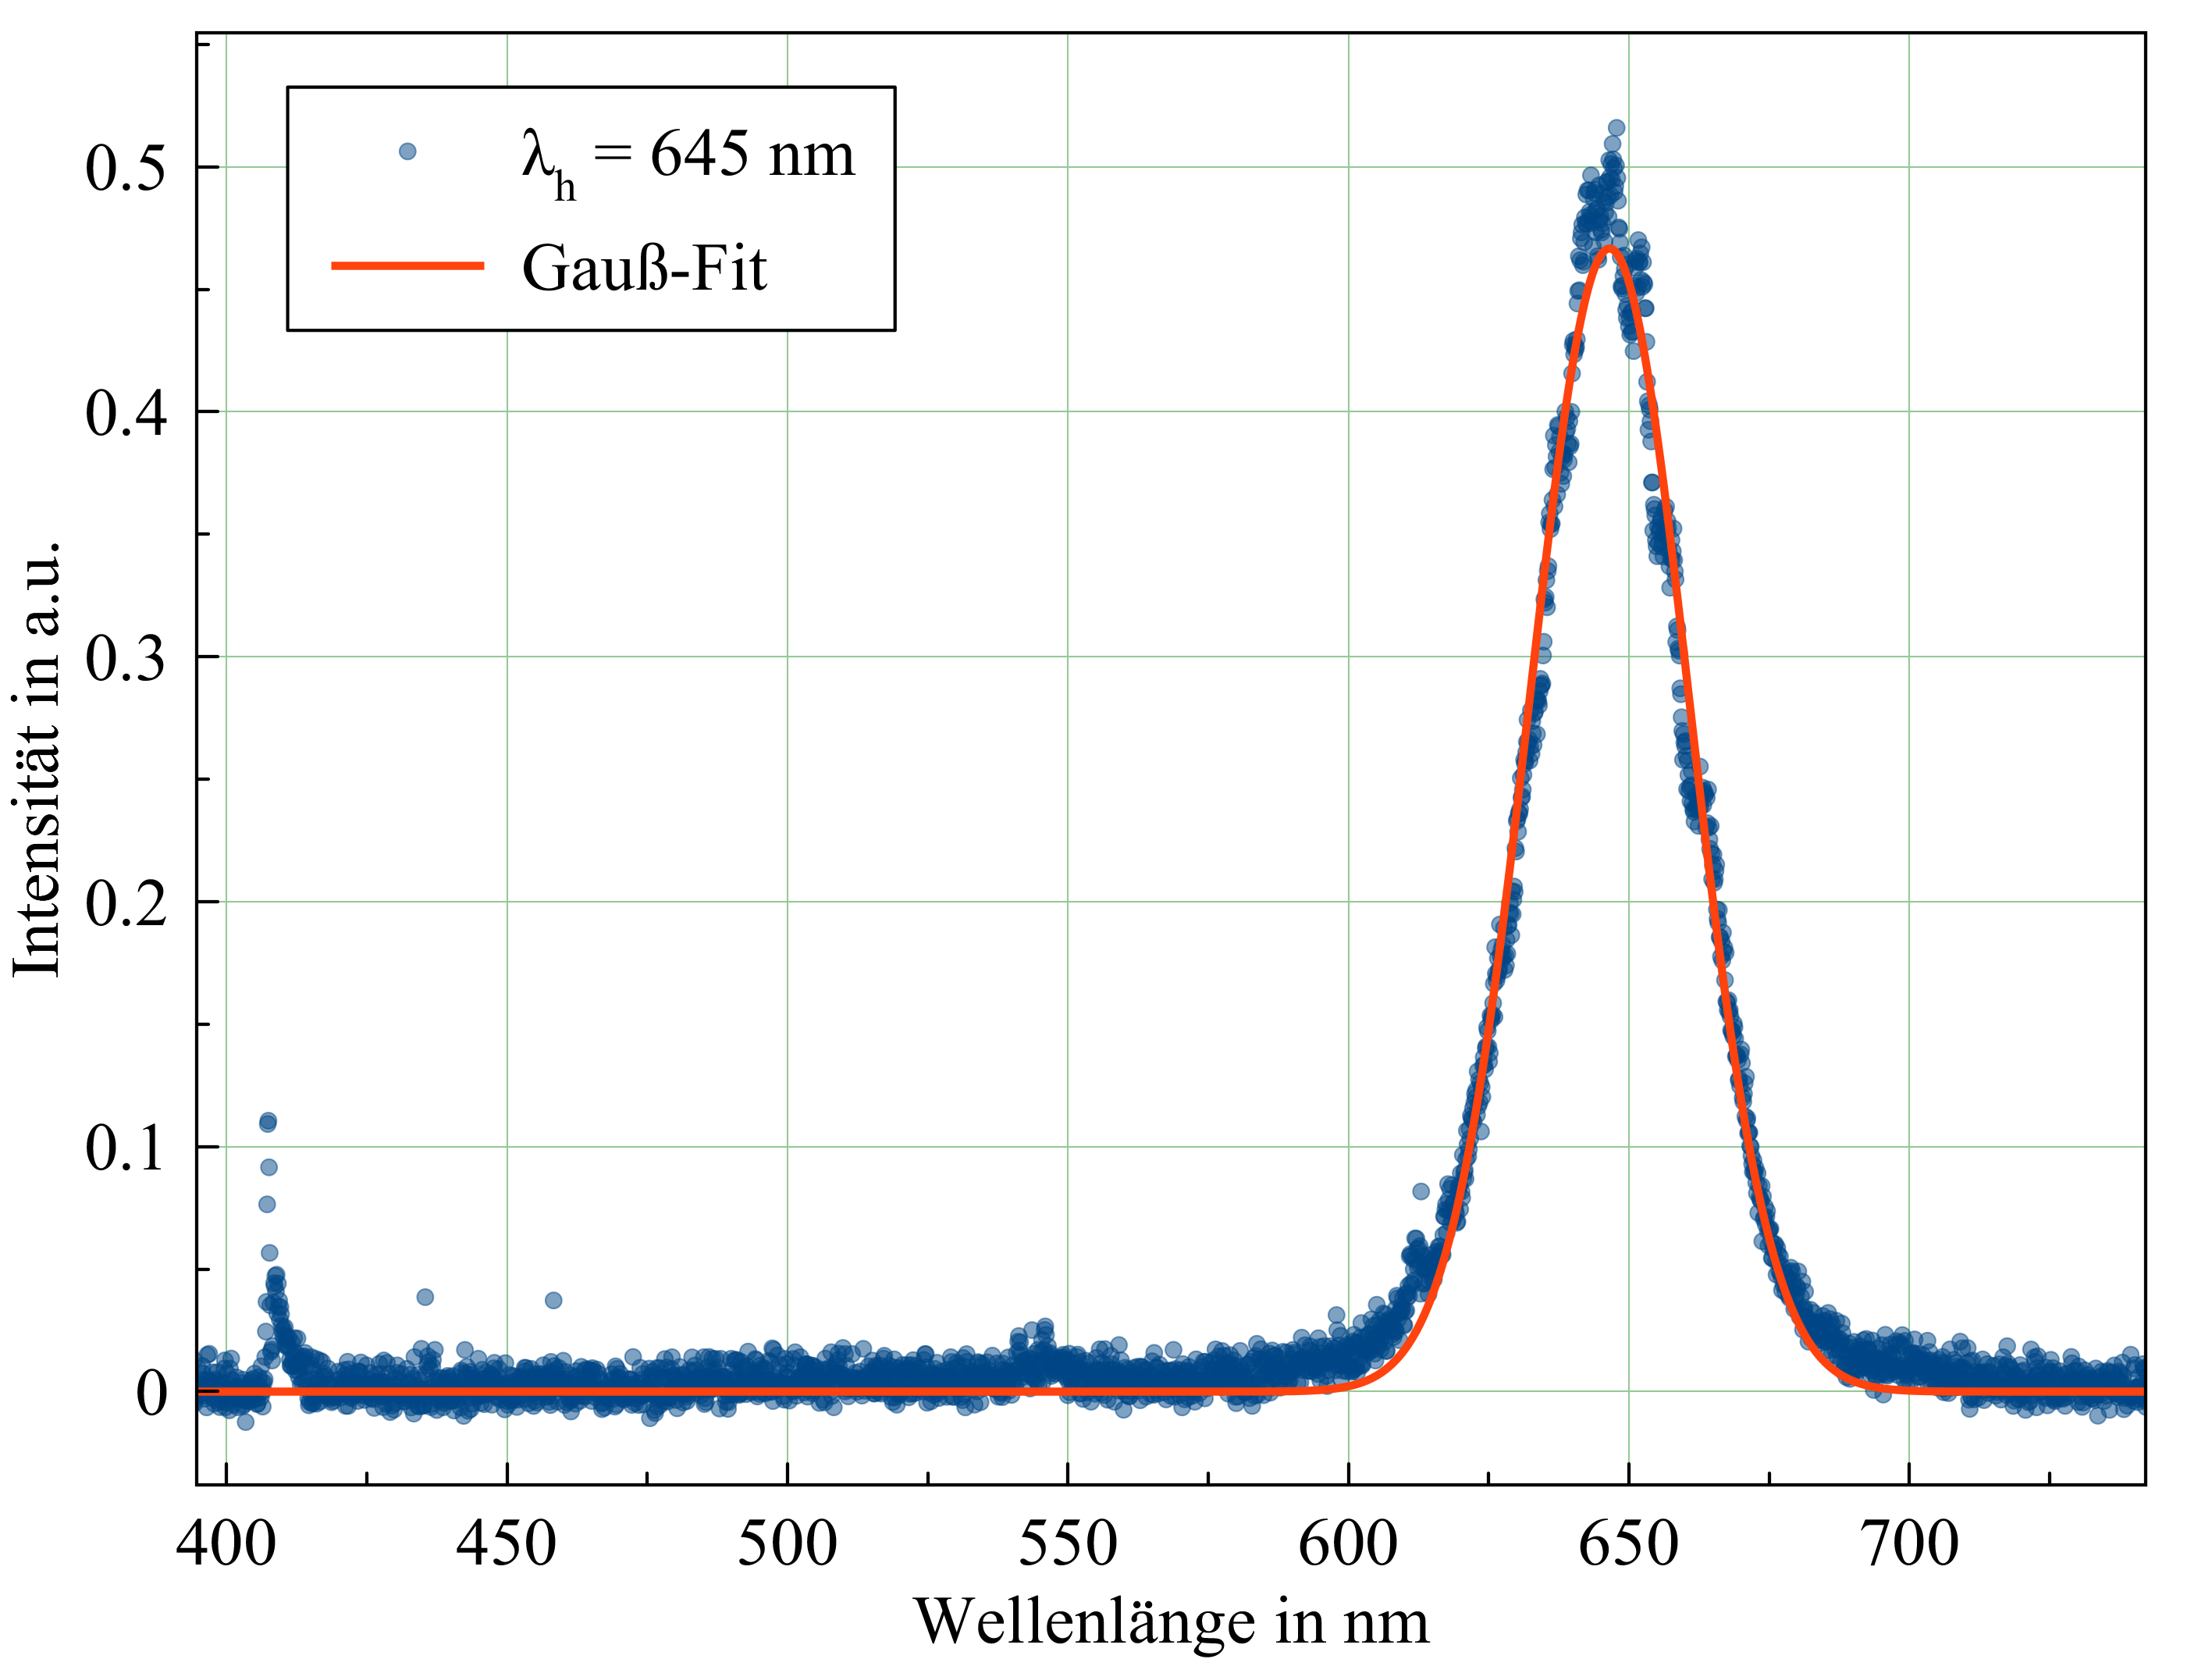
\includegraphics[width=0.7\textwidth]{plots/PL_645nm.png}
  \caption{Photolumineszenzspektrum einer Probe mit Emissionswellenlänge $\lambda_{\text{PL}}=\SI{645}{\nano\meter}$ bei einer Anregungswellenlänge von $\lambda=\SI{405}{\nano\meter}$ und einer Eingangsleistung von $\SI{130}{\milli\watt}$.}
  \label{fig:pl645}
\end{figure}
\begin{figure}[H]
  \centering
  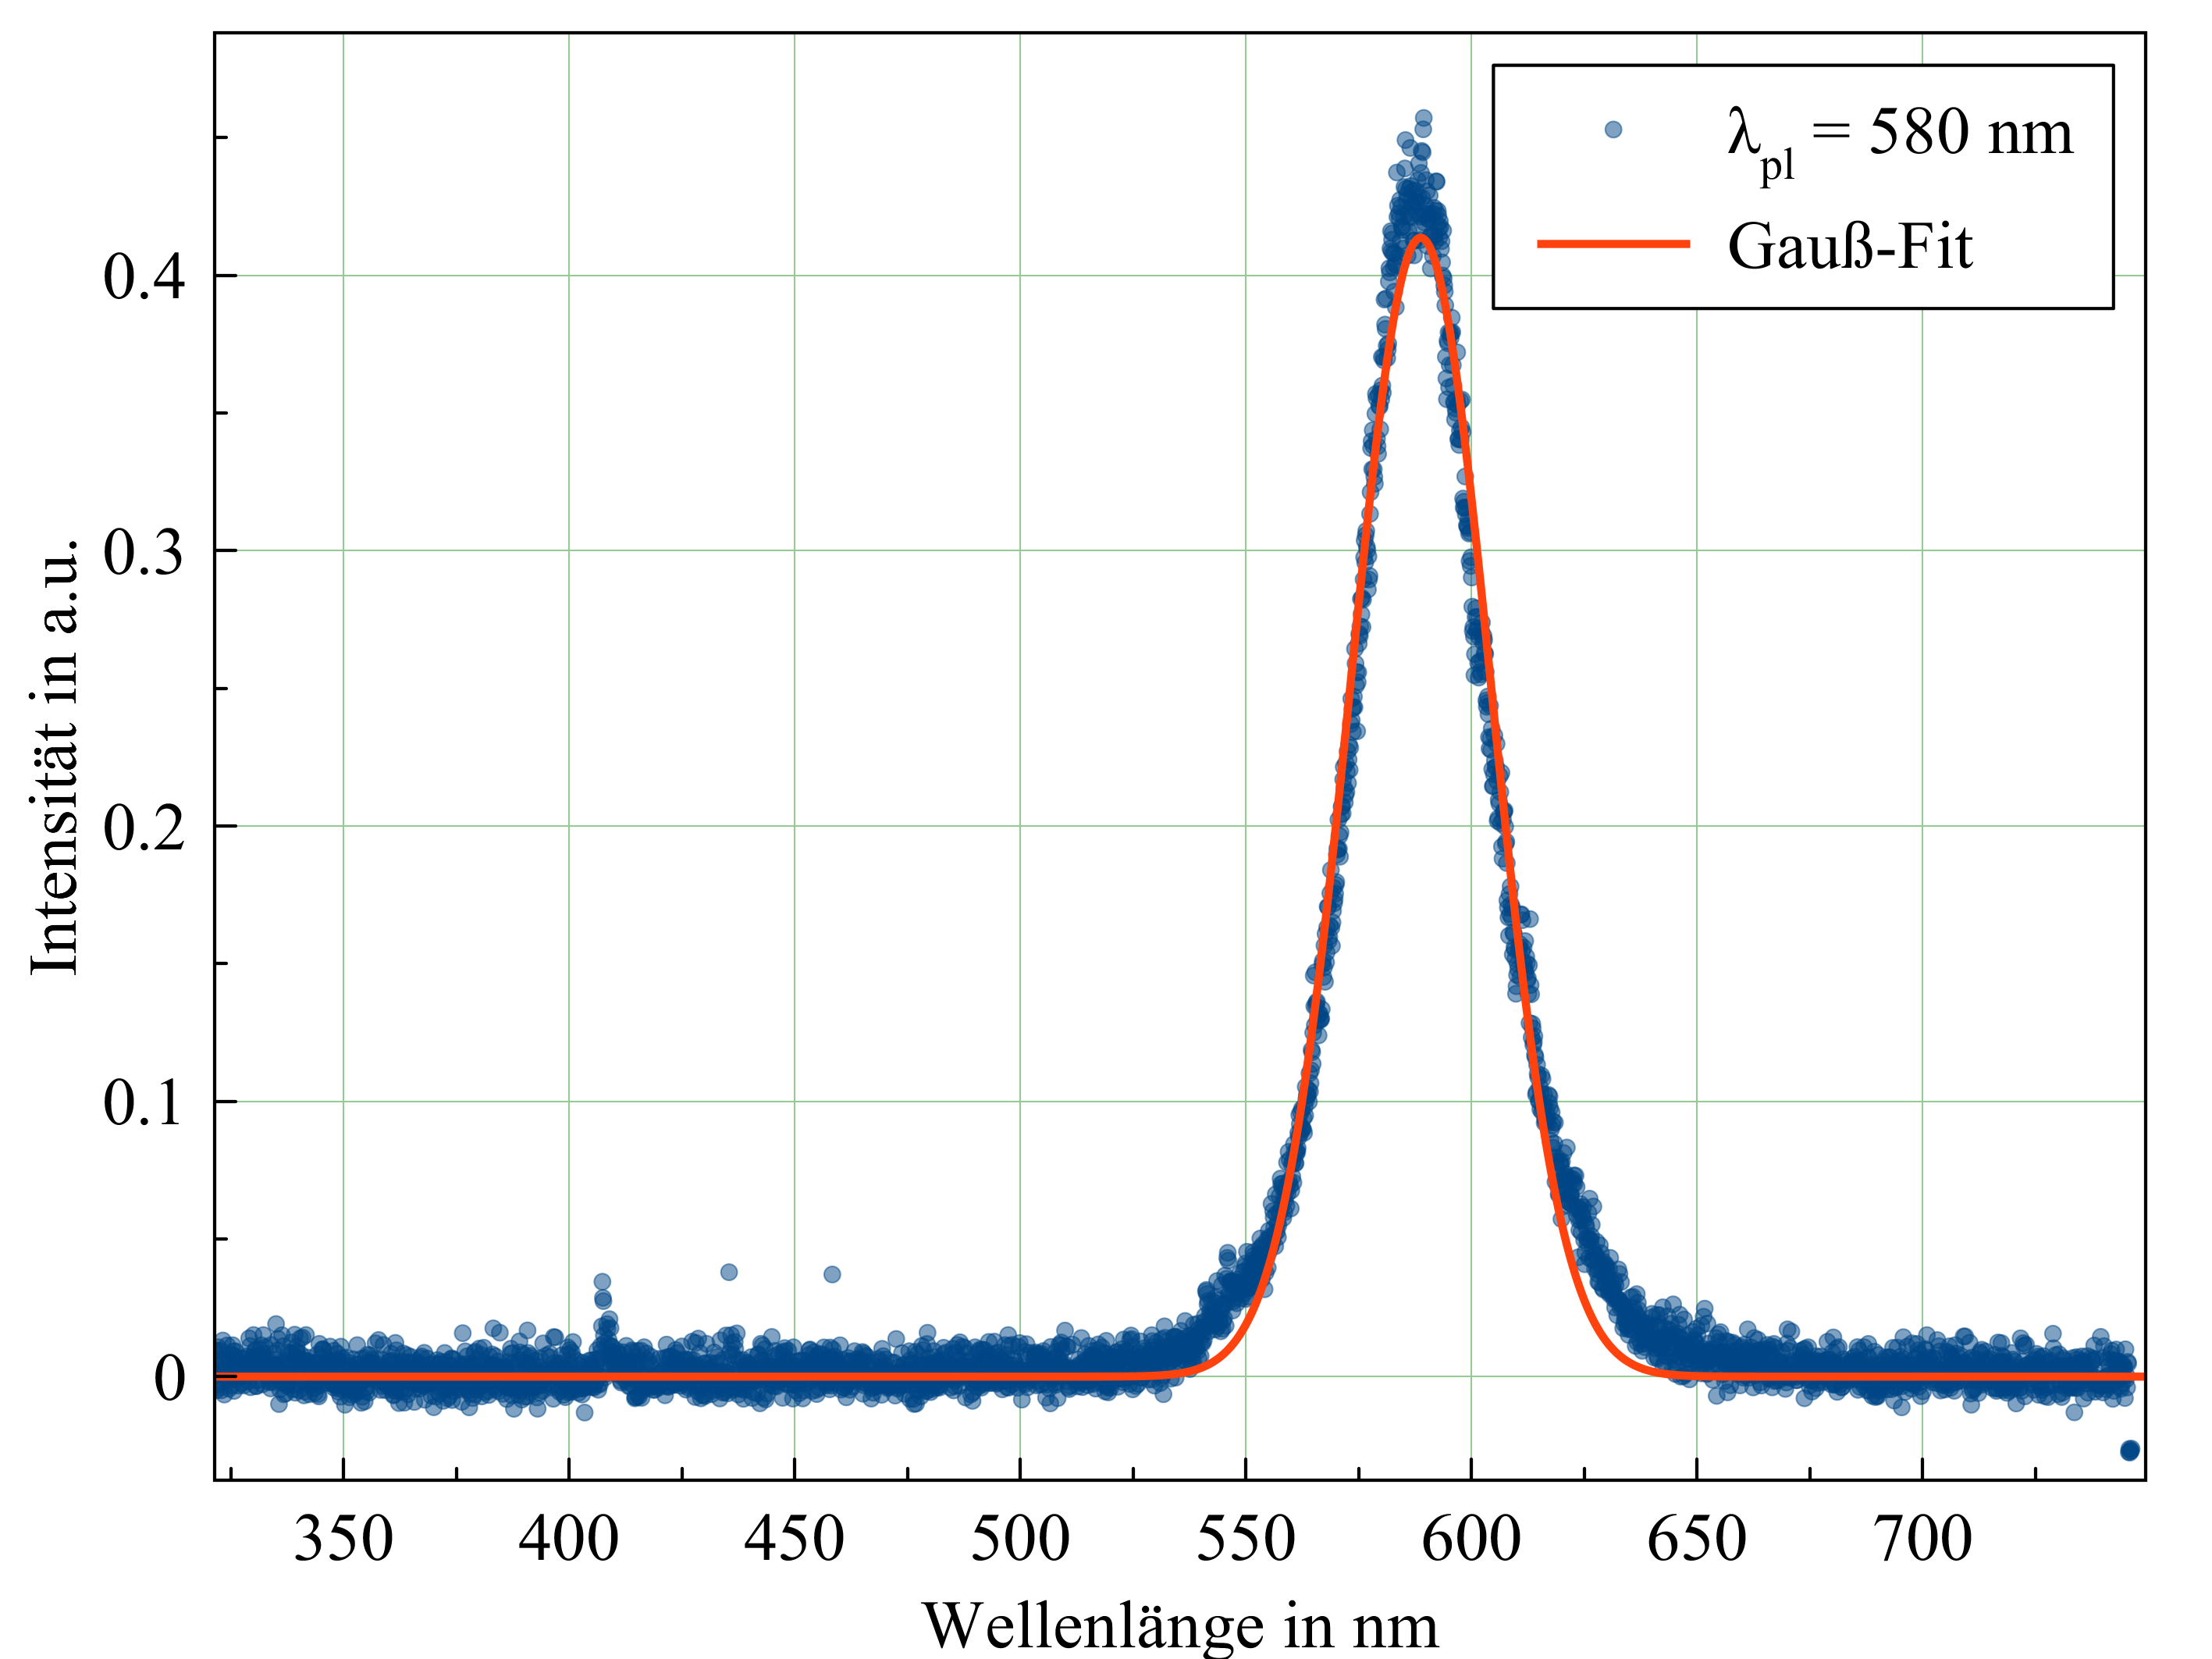
\includegraphics[width=0.7\textwidth]{plots/PL_580nm.png}
  \caption{Photolumineszenzspektrum einer Probe mit Emissionswellenlänge $\lambda_{\text{PL}}=\SI{580}{\nano\meter}$ bei einer Anregungswellenlänge von $\lambda=\SI{405}{\nano\meter}$ und einer Eingangsleistung von $\SI{130}{\milli\watt}$.}
  \label{fig:pl580}
\end{figure}
\begin{figure}[H]
  \centering
  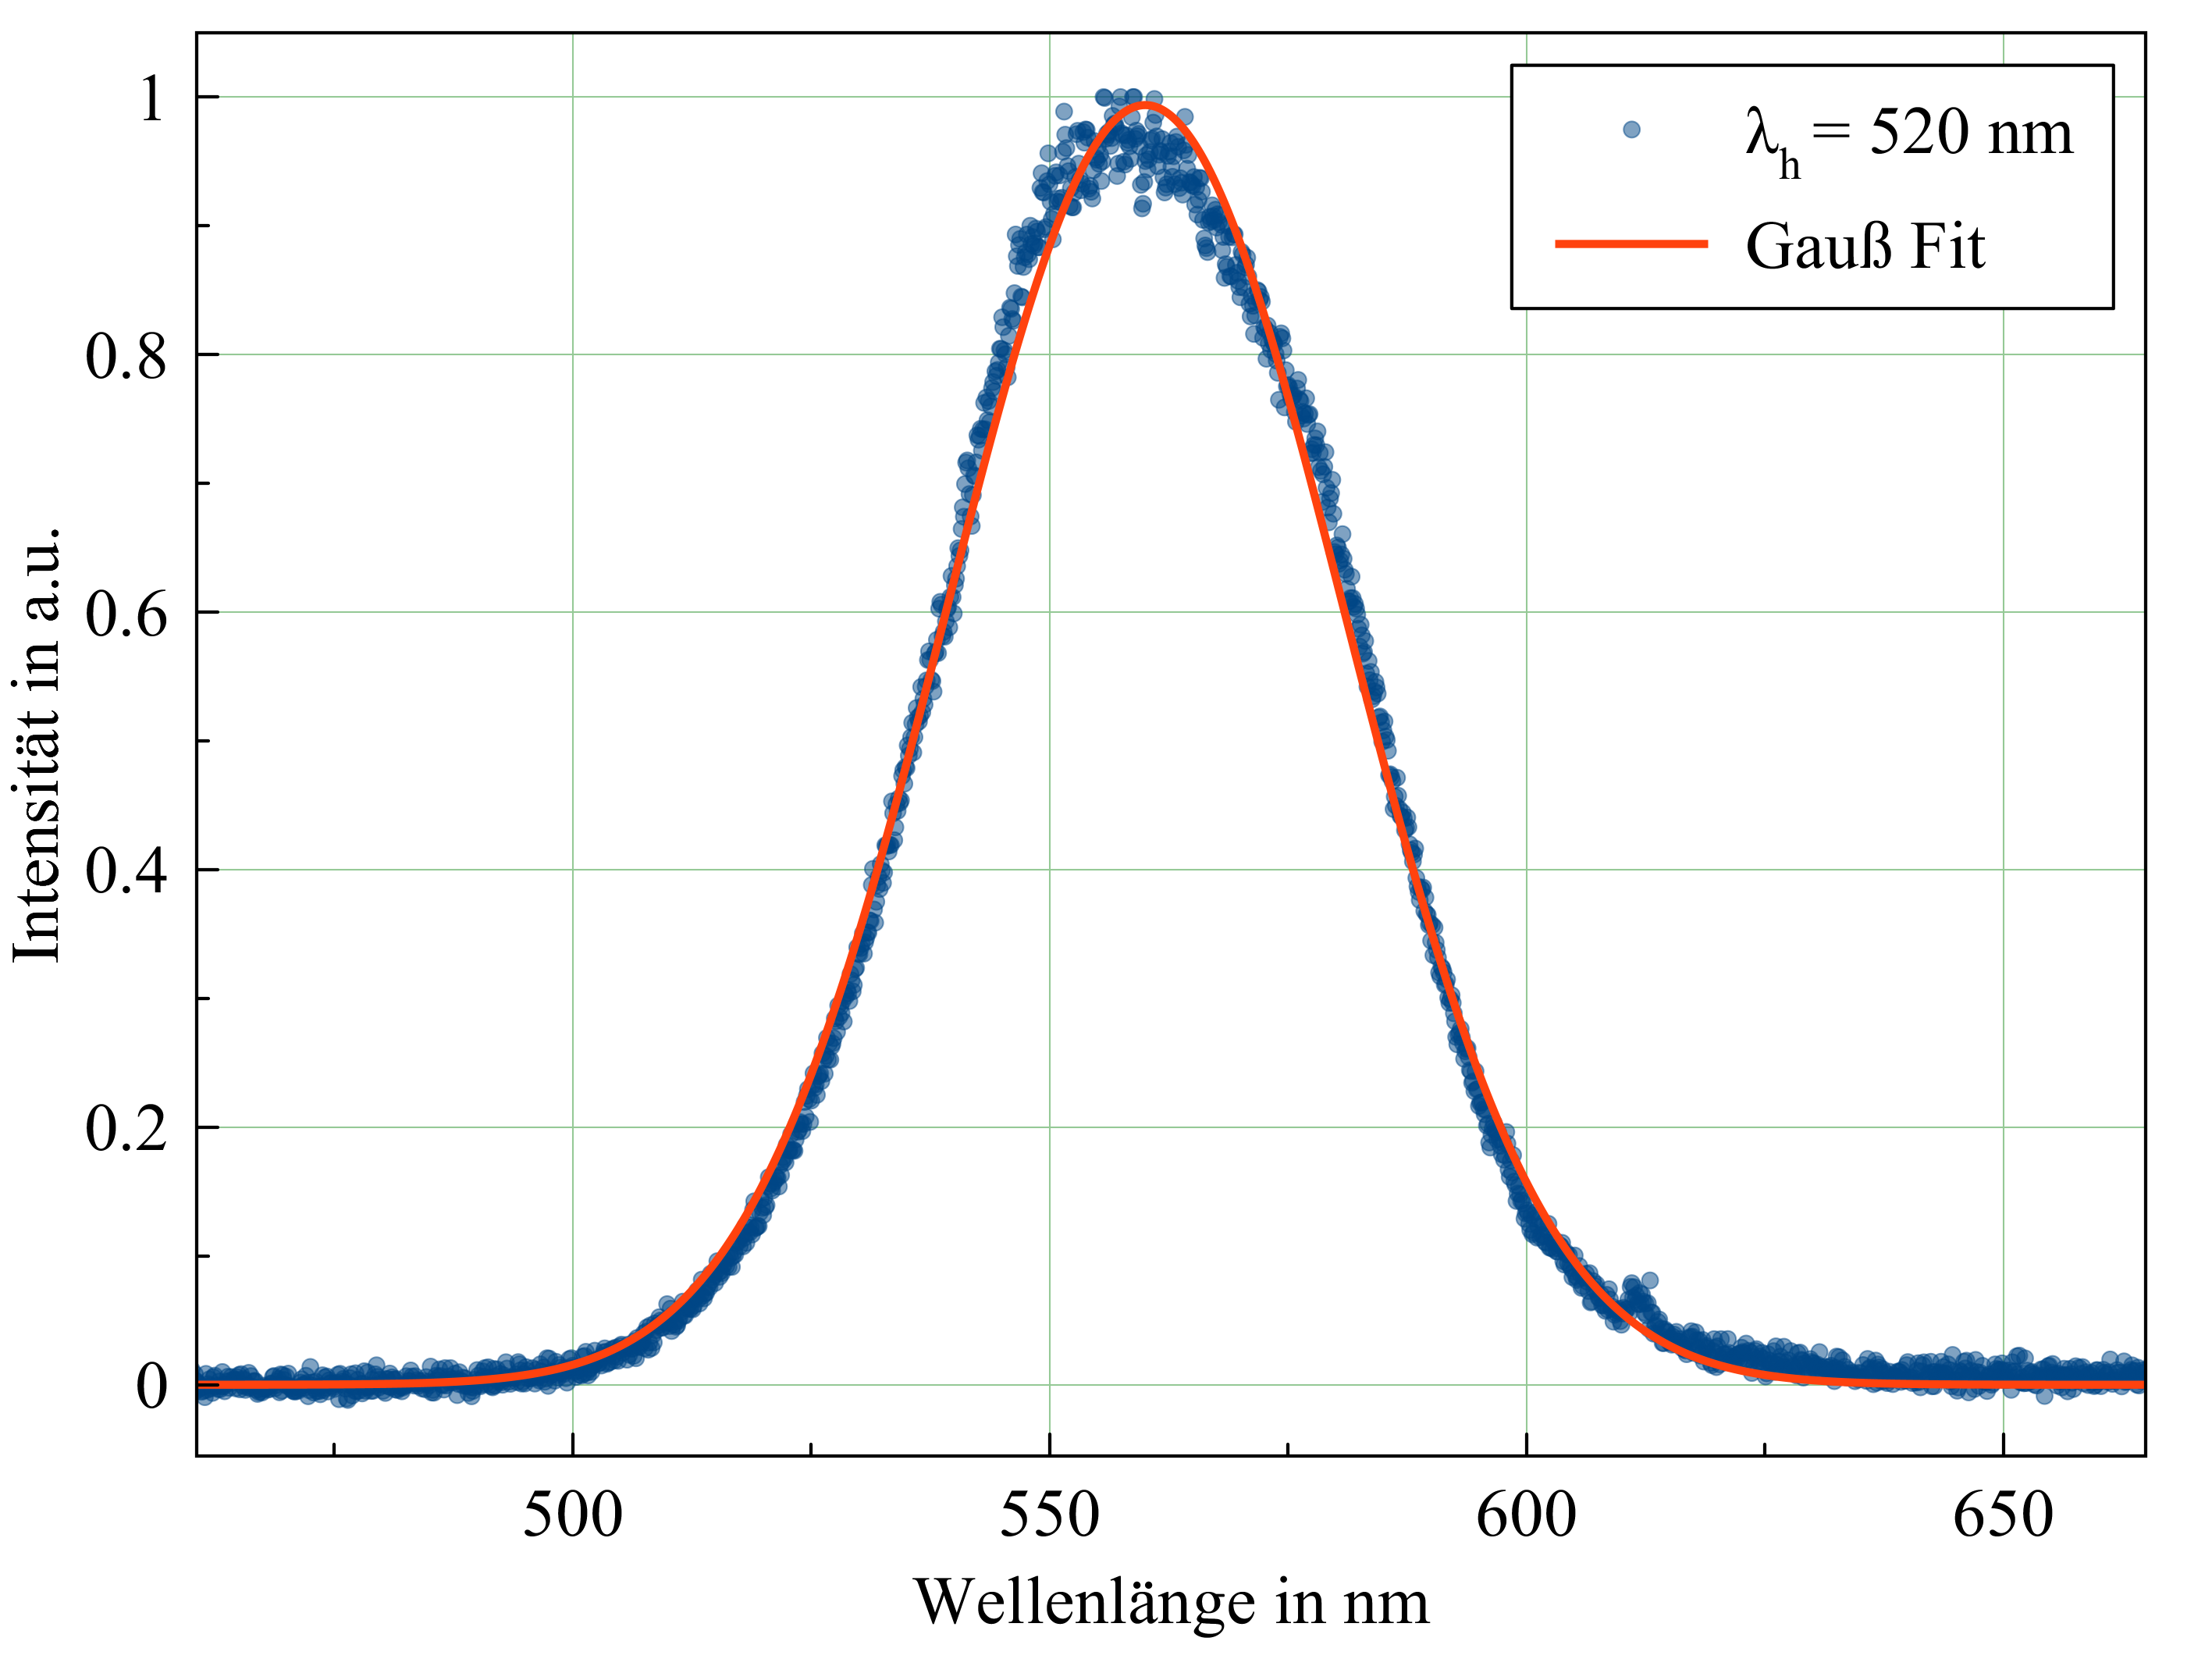
\includegraphics[width=0.7\textwidth]{plots/PL_520nm.png}
  \caption{Photolumineszenzspektrum einer Probe mit Emissionswellenlänge $\lambda_{\text{PL}}=\SI{520}{\nano\meter}$ bei einer Anregungswellenlänge von $\lambda=\SI{405}{\nano\meter}$ und einer Eingangsleistung von $\SI{1,5}{\milli\watt}$.}
  \label{fig:pl520}
\end{figure}

Mithilfe der Formel \ref{eq: E_R} aus Kapitel \ref{sec:theo} wird die Ausdehnung der Quantenpunkte ermittelt. Die Ergebnisse der Abschätzung sind in Tabelle \ref{tab:breiten} einzusehen.
\begin{table}[H]
  \centering
  \caption{Aus der Photolumineszenzwellenlänge $\lambda_{\text{pl}}$ berechnete Ausdehnung $a$ der Quantenpunkte.}
  \label{tab:breiten}
  \begin{tabular}{cc}
    \toprule
     $\lambda_{\text{pl}}$ in $\si{\nano\meter}$& $a$ in $\si{\nano\meter}$ \\
    \midrule
    520 & 2.63 \\
    580 & 3.51 \\
    645 & 6.47 \\
    \bottomrule
  \end{tabular}
\end{table}

Die zur Berechnung der Ausdehnung verwendeten Materialparameter sind in Tabelle \ref{tab:const} zusammengestellt.
\begin{table}[H]
  \centering
  \caption{Zur Abschätzung der Ausdehnung benötigte Materialkonstanten. \cite{dissArens}}
  \label{tab:const}
  \begin{tabular}{c|c}
    \toprule
    $\epsilon_r $ & $ 9.15$ \\
    $m^*_h$ & $ -0.45 m_0$ \\
    $m^*_e $ & $ 0.15 m_0$ \\
    $E_g $ & $\SI{1.84}{\electronvolt}$ \\
    \bottomrule
  \end{tabular}
\end{table}
Dabei wurden die effektiven Massen der Ladungsträger und die Permittivität für eine Bewegung senkrecht zur ausgezeichneten Achse verwendet.

\newpage
\subsection{Abhängigkeit der PL von der Eingangsleistung}
\label{sec:leistung}
Die Resultate der Untersuchung der Leistungsabhängigkeit sind in den Abbildungen ~\ref{fig:Podep520} und ~\ref{fig:Podep645} für zwei der Proben graphisch dargestellt. Es ist zunächst ein linearer Anstieg zu sehen, welcher in eine Sättigung bei höheren Eingangsleistungen übergeht. Der untersuchte Bereich der Leistung ist für die in Abbildung \ref{fig:Podep520} gezeigte Probe deutlich kleiner, da die Photodiode eher in Sättigung geht.
\begin{figure}[H]
  \centering
  \begin{subfigure}{0.5\textwidth}
    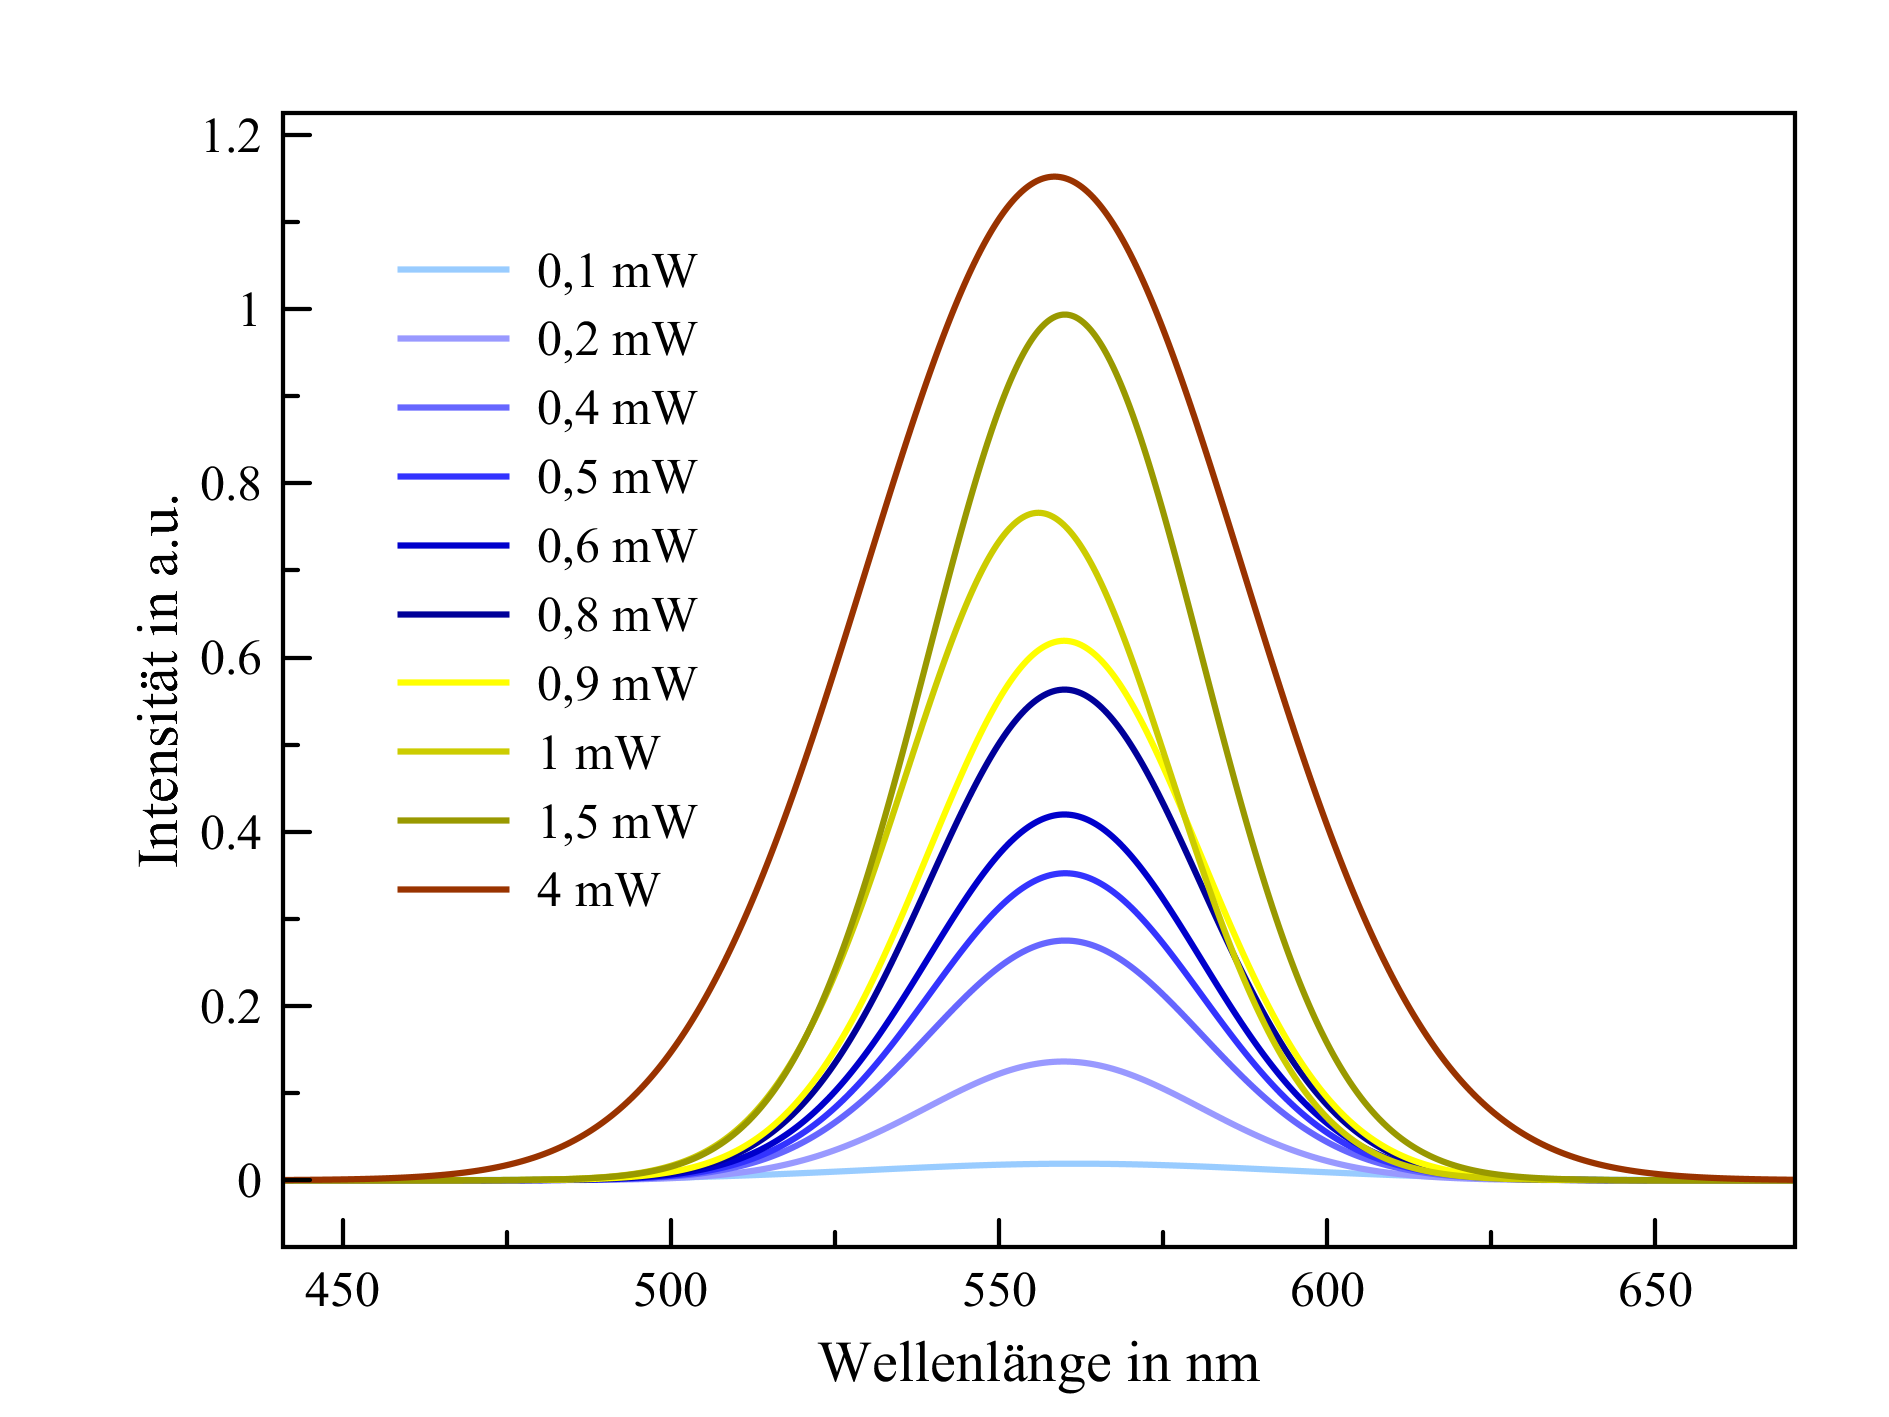
\includegraphics[width=\textwidth]{plots/Powerdependence_520nm.png}
  \end{subfigure}
  \begin{subfigure}{0.45\textwidth}
    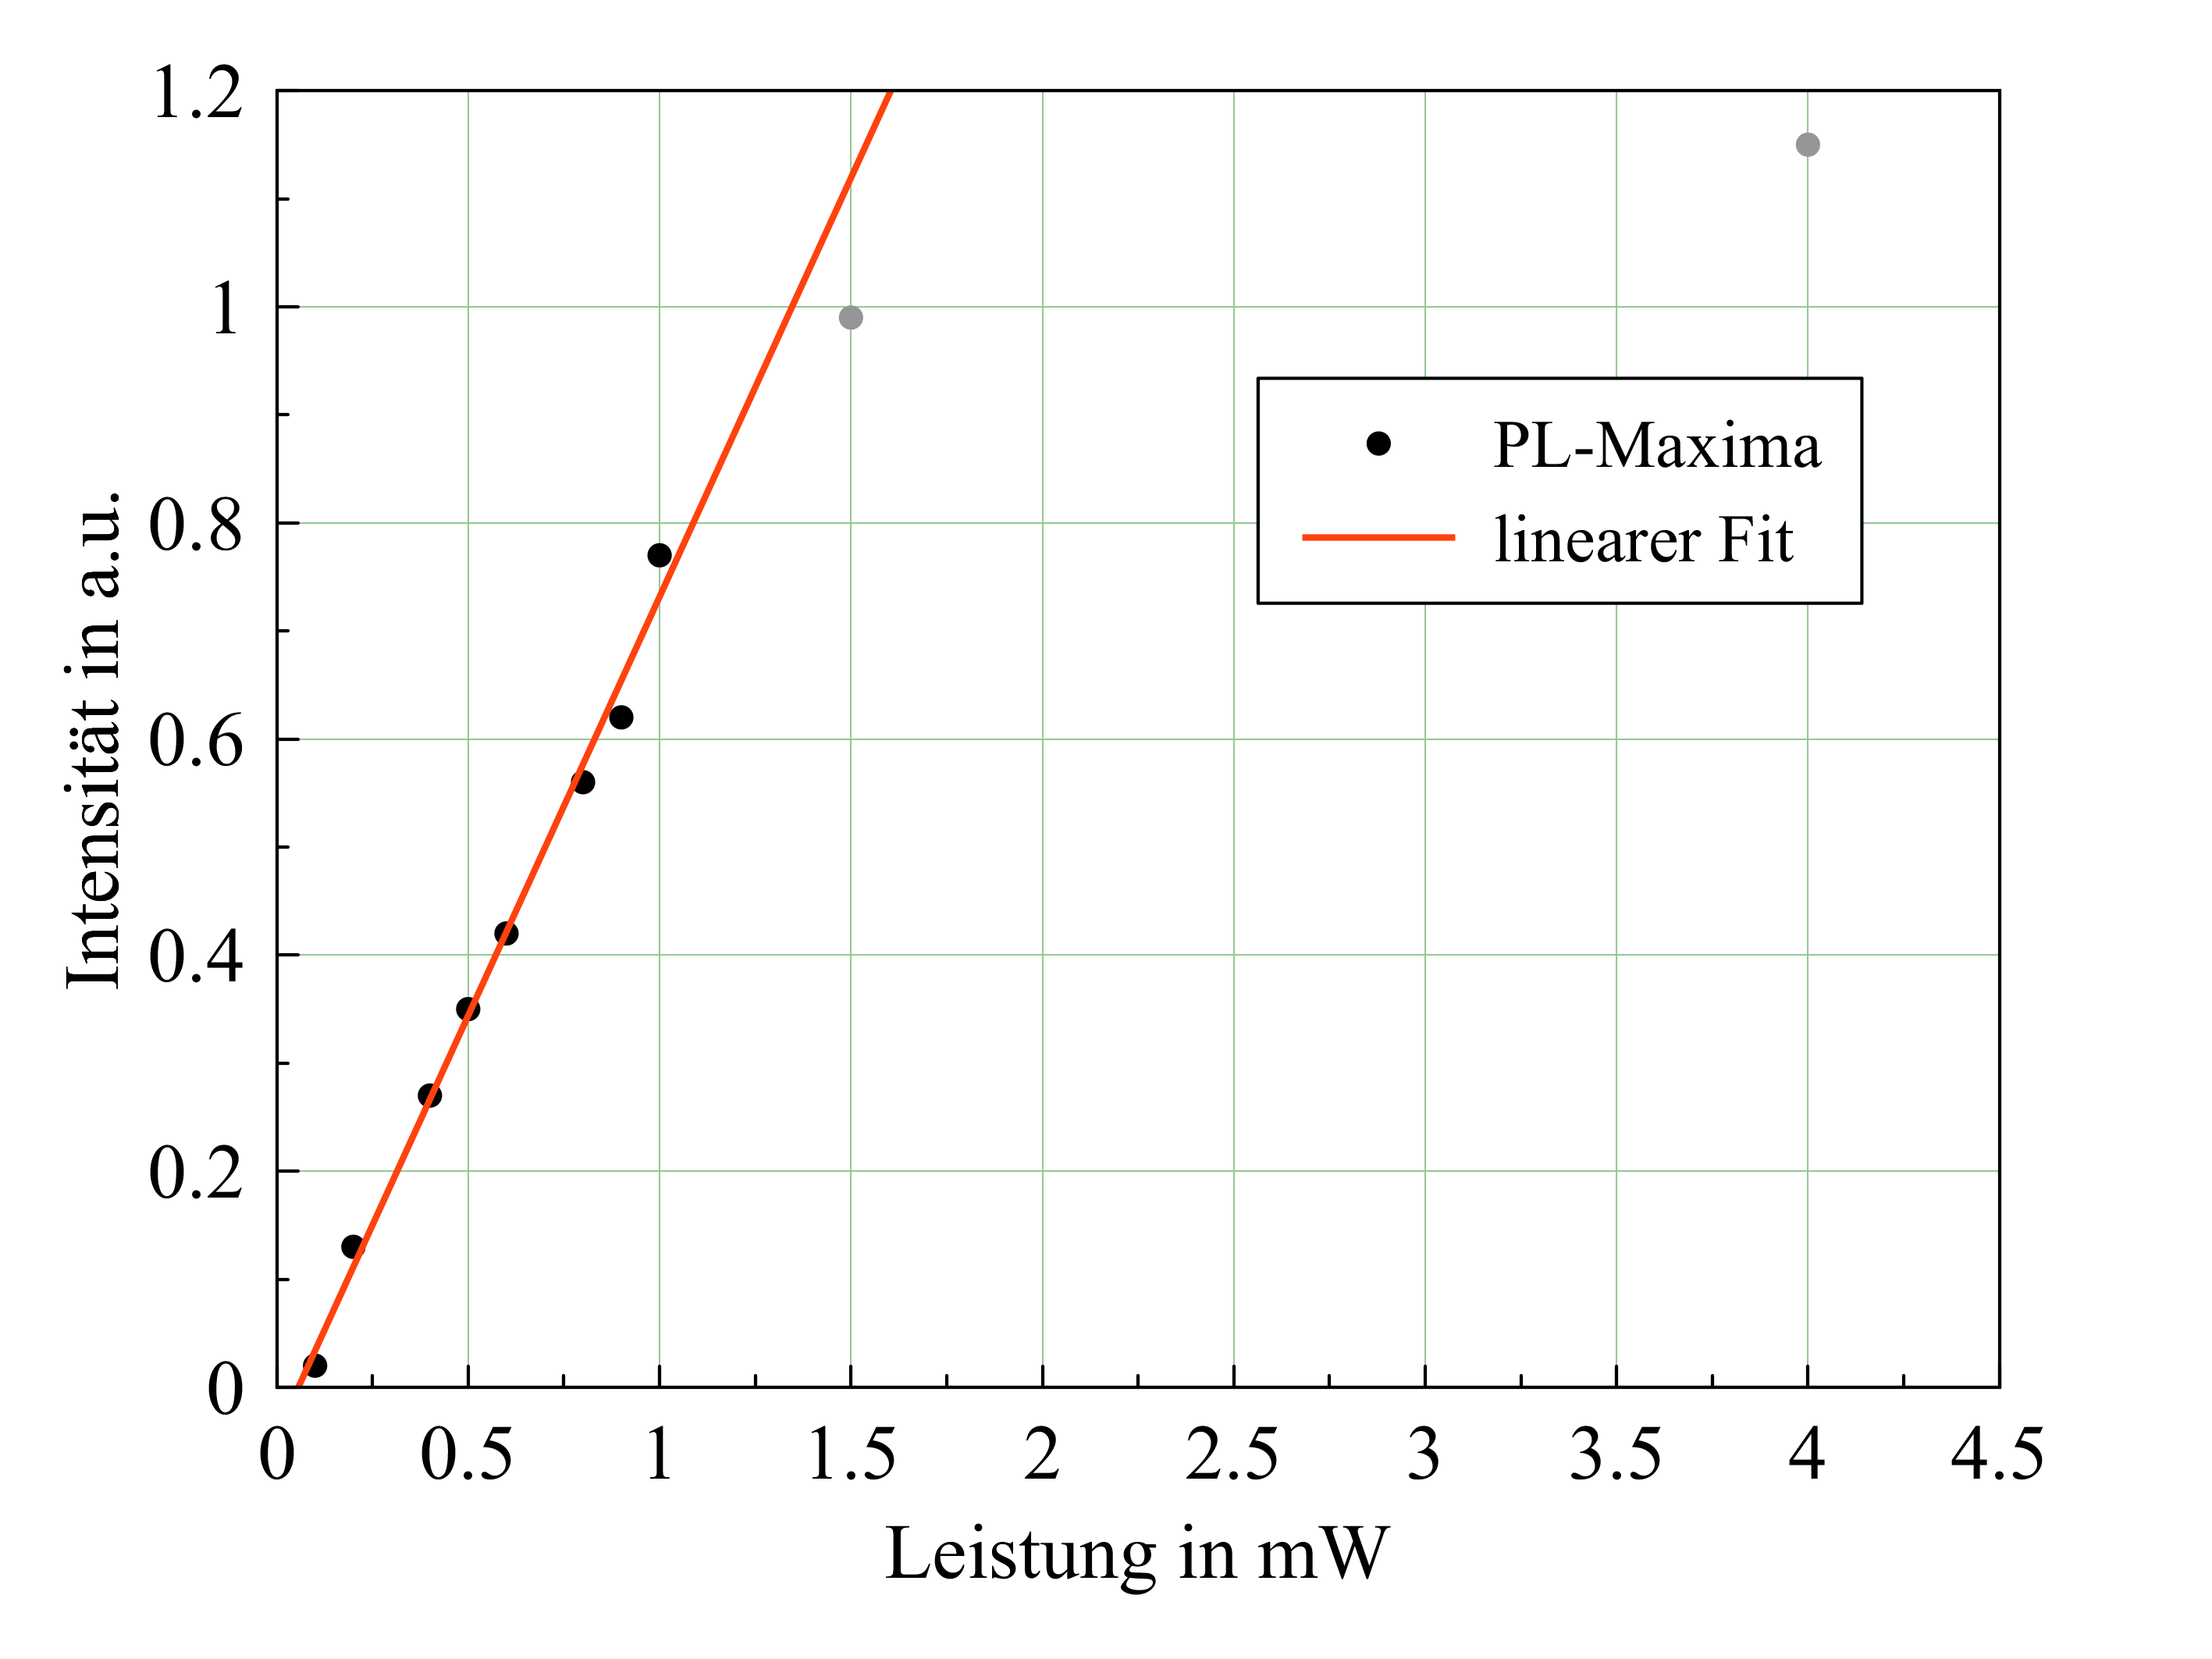
\includegraphics[width=\textwidth]{plots/Powerdepfit_520.png}
  \end{subfigure}
  \caption{Abhängigkeit der Photolumineszenz von der Eingangsleistung für eine Probe mit PL-Wellenlänge $\lambda_{\text{pl}} = \SI{520}{\nano\meter}$.
  \textbf{Links:} Kurvenschar der Ausgleichsrechnungen der PL-Spektren für unterschiedliche Leistungen. \textbf{Rechts:} Darstellung der Maxima der Ausgleichskurven und Fit des linearen Anstiegs.}
  \label{fig:Podep520}
\end{figure}
\begin{figure}[H]
  \centering
  \begin{subfigure}{0.49\textwidth}
    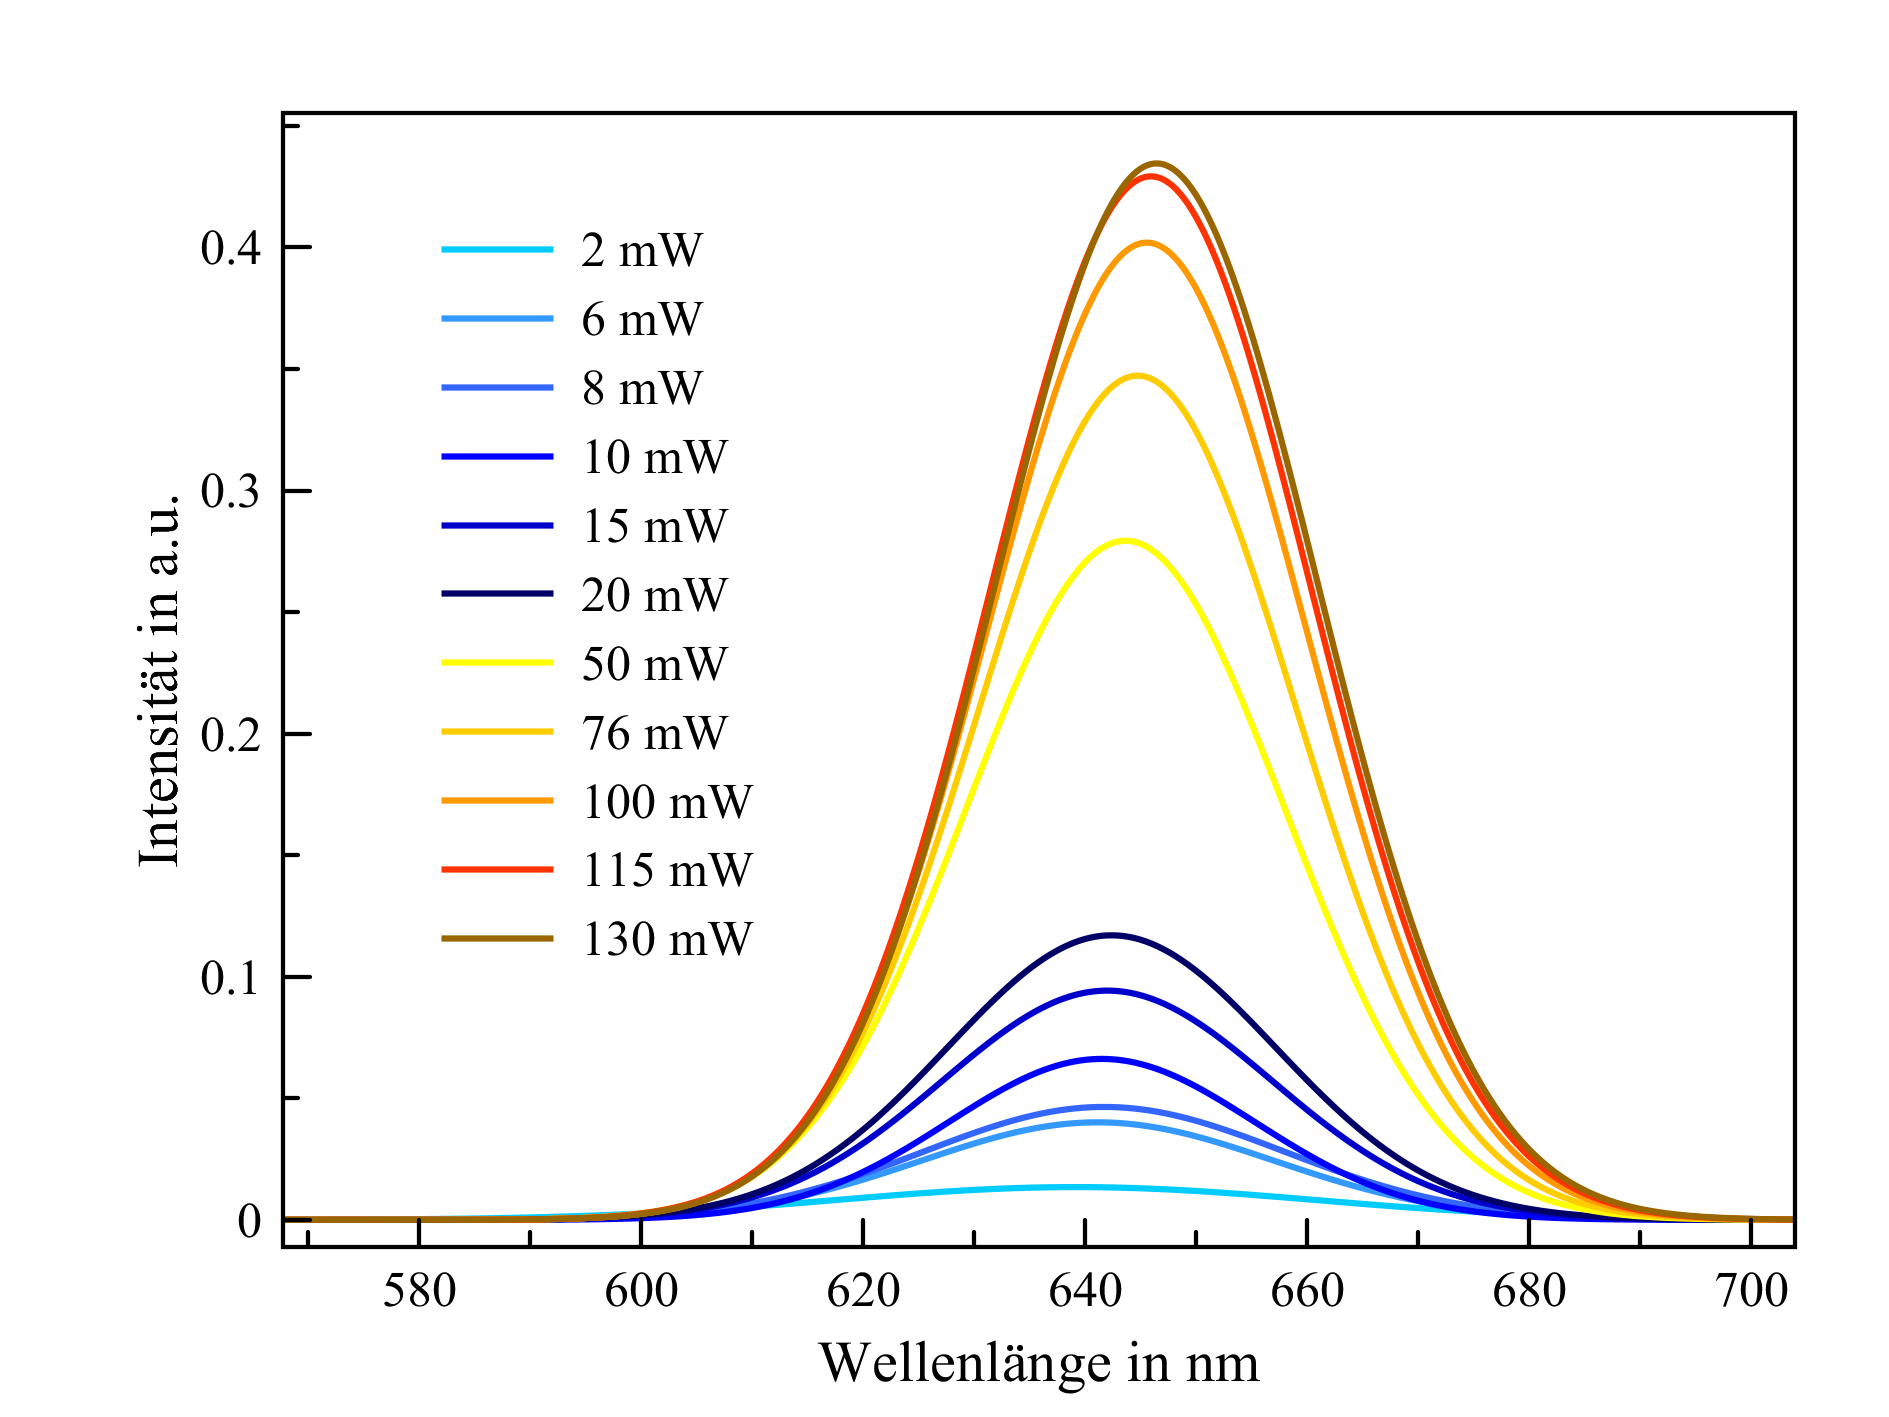
\includegraphics[width=\textwidth]{plots/Powerdependence_645nm.png}
  \end{subfigure}
  \begin{subfigure}{0.46\textwidth}
    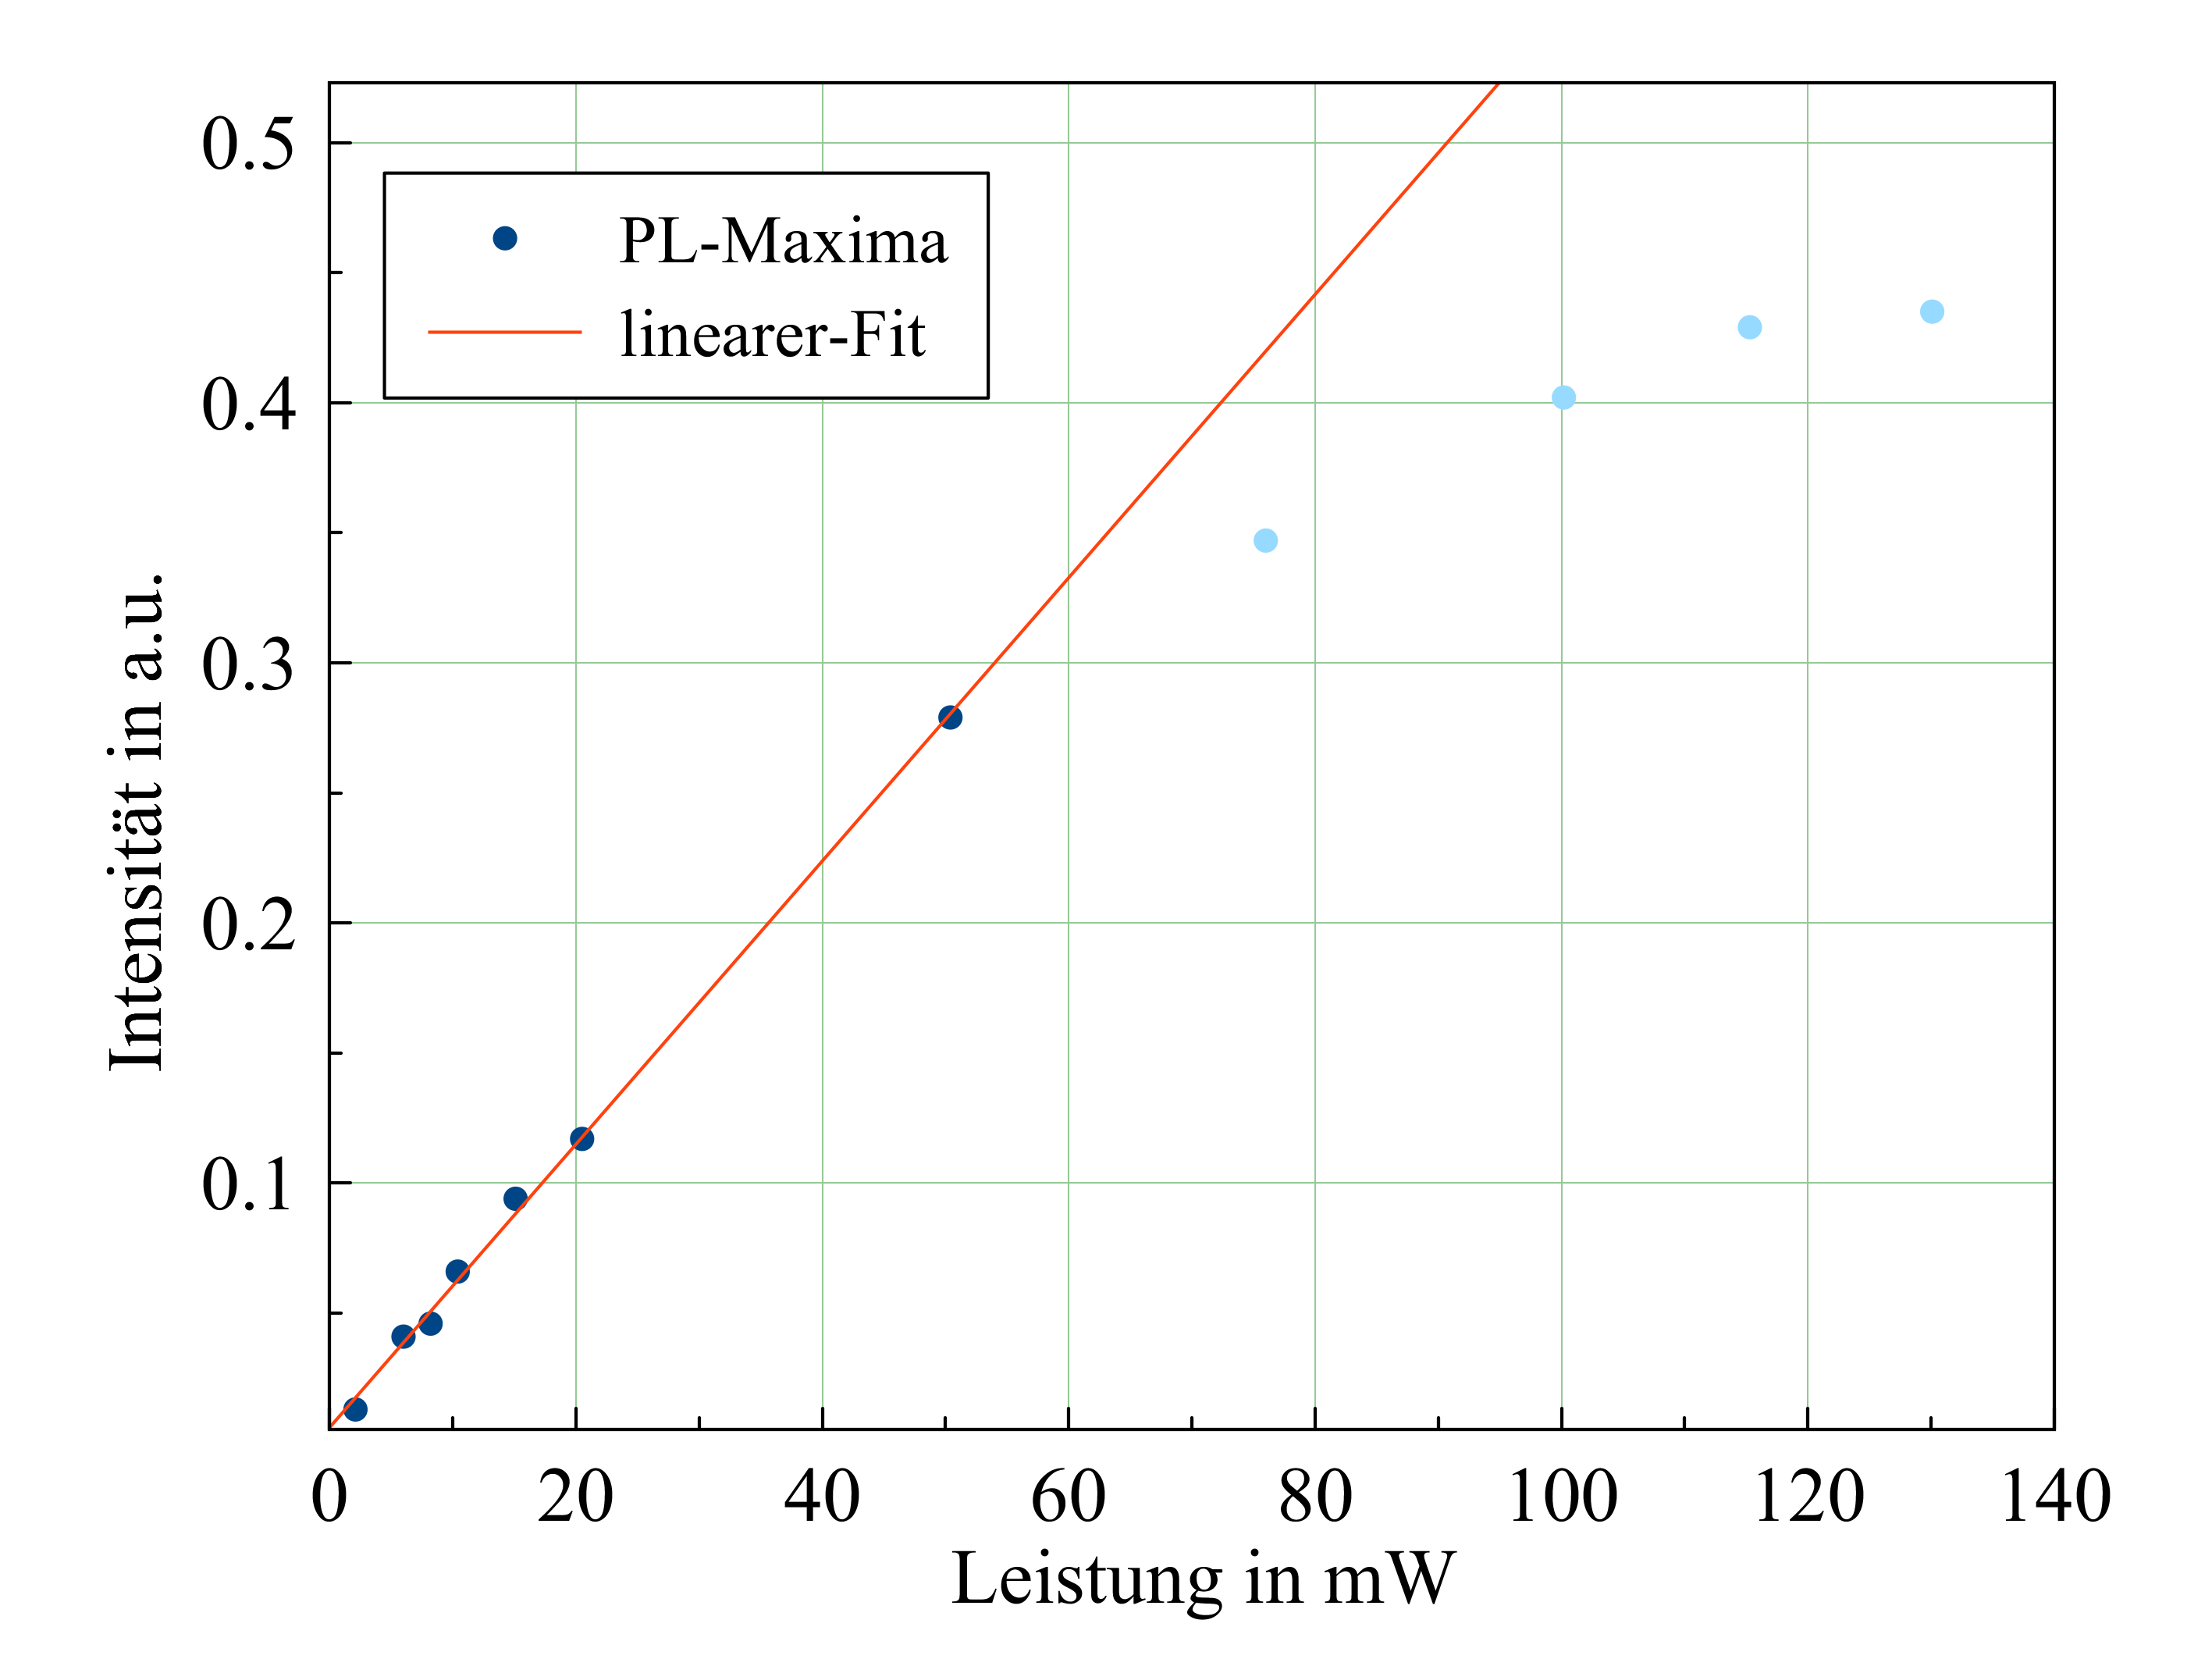
\includegraphics[width=\textwidth]{plots/Powerdepfit_645.png}
  \end{subfigure}
  \caption{Abhängigkeit der Photolumineszenz von der Eingangsleistung für eine Probe mit PL-Wellenlänge $\lambda_{\text{pl}} = \SI{645}{\nano\meter}$. \textbf{Links:} Kurvenschar der Ausgleichsrechnungen der PL-Spektren für unterschiedliche Leistungen. \textbf{Rechts:} Darstellung der Maxima der Ausgleichskurven und Fit des linearen Anstiegs.}
  \label{fig:Podep645}
\end{figure}

Weiterhin sind Schwankungen der Position der maximalen Emissionsenergie der Photolumineszenz auffällig. Die Position der maximalen Emissionsenergie ist für beide Messungen in Abbildung \ref{fig:posem} aufgetragen. Es zeigt sich ein klarer Anstieg der Emissionswellenlänge für die $\lambda_{\text{pl}}=\SI{645}{\nano\meter}$ Probe. Aus den Ergebnissen der Messungen an der $\lambda_{\text{pl}}=\SI{520}{\nano\meter}$ lassen sich keine klaren Abhängigkeiten ableiten.
\begin{figure}[H]
  \centering
  \begin{subfigure}{0.49\textwidth}
    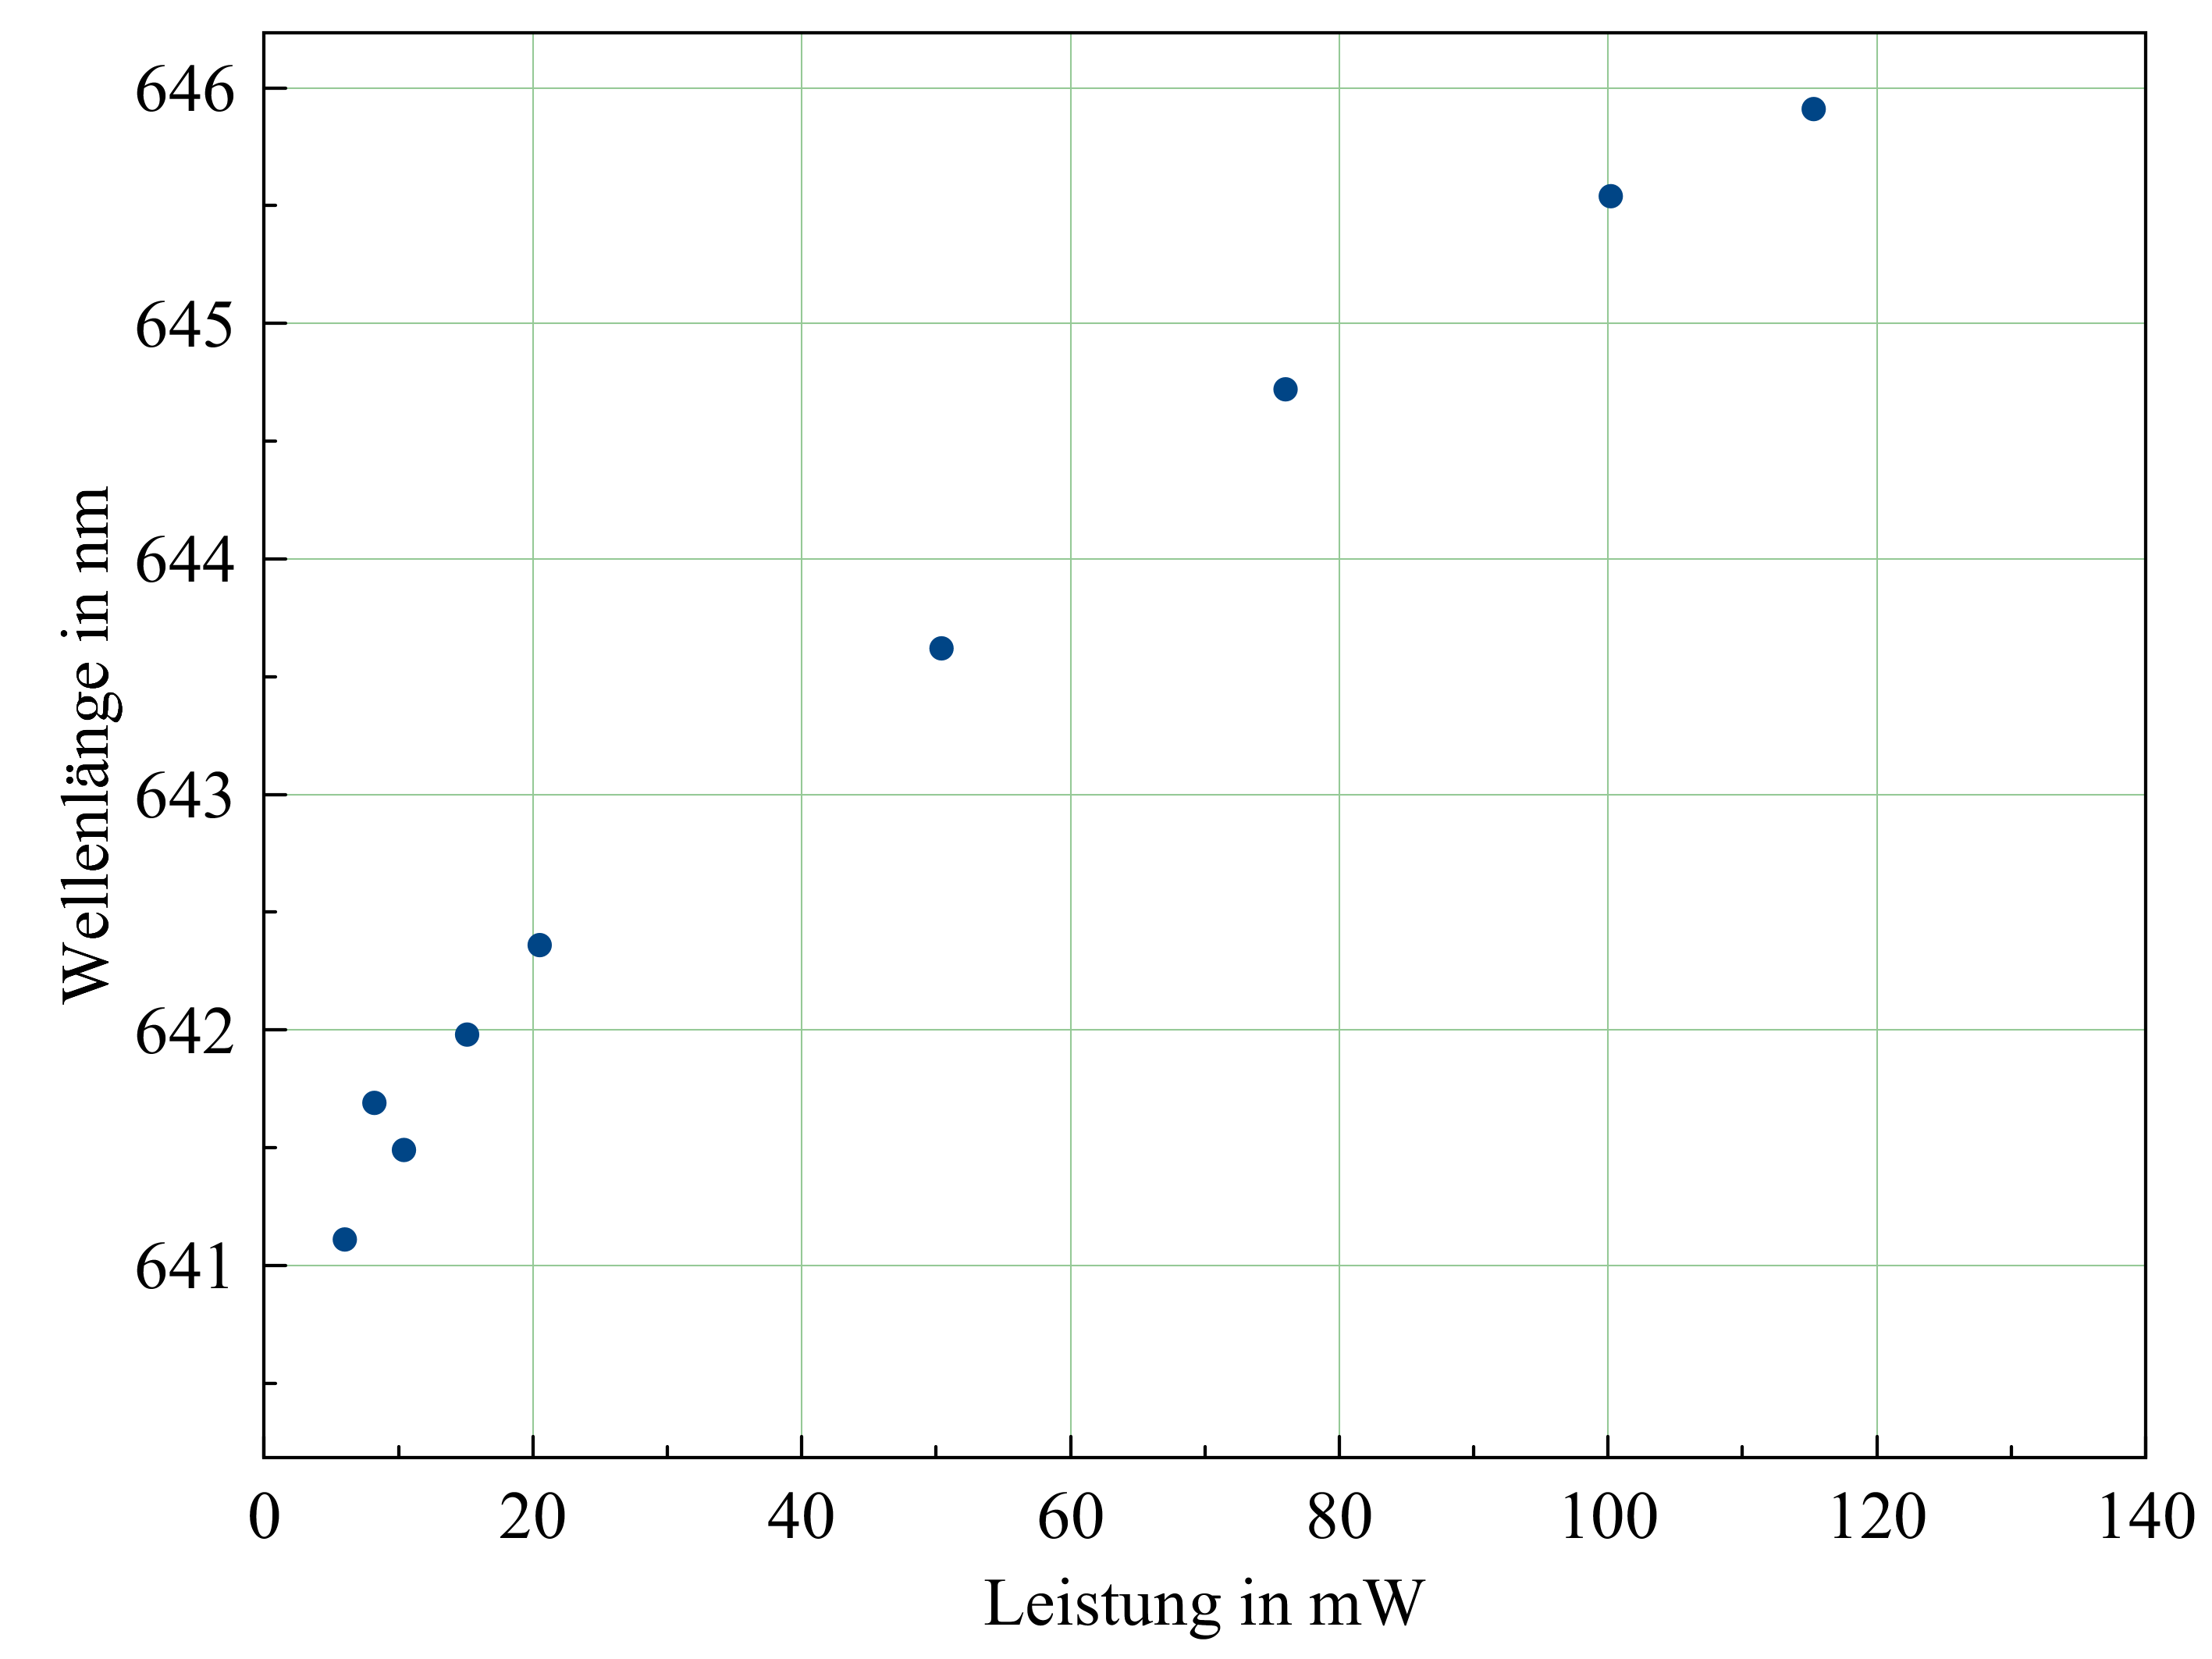
\includegraphics[width=\textwidth]{plots/posemplot_645nm.png}
    \caption{$\lambda_{\text{pl}} = \SI{645}{\nano\meter}$}
  \end{subfigure}
  \begin{subfigure}{0.49\textwidth}
    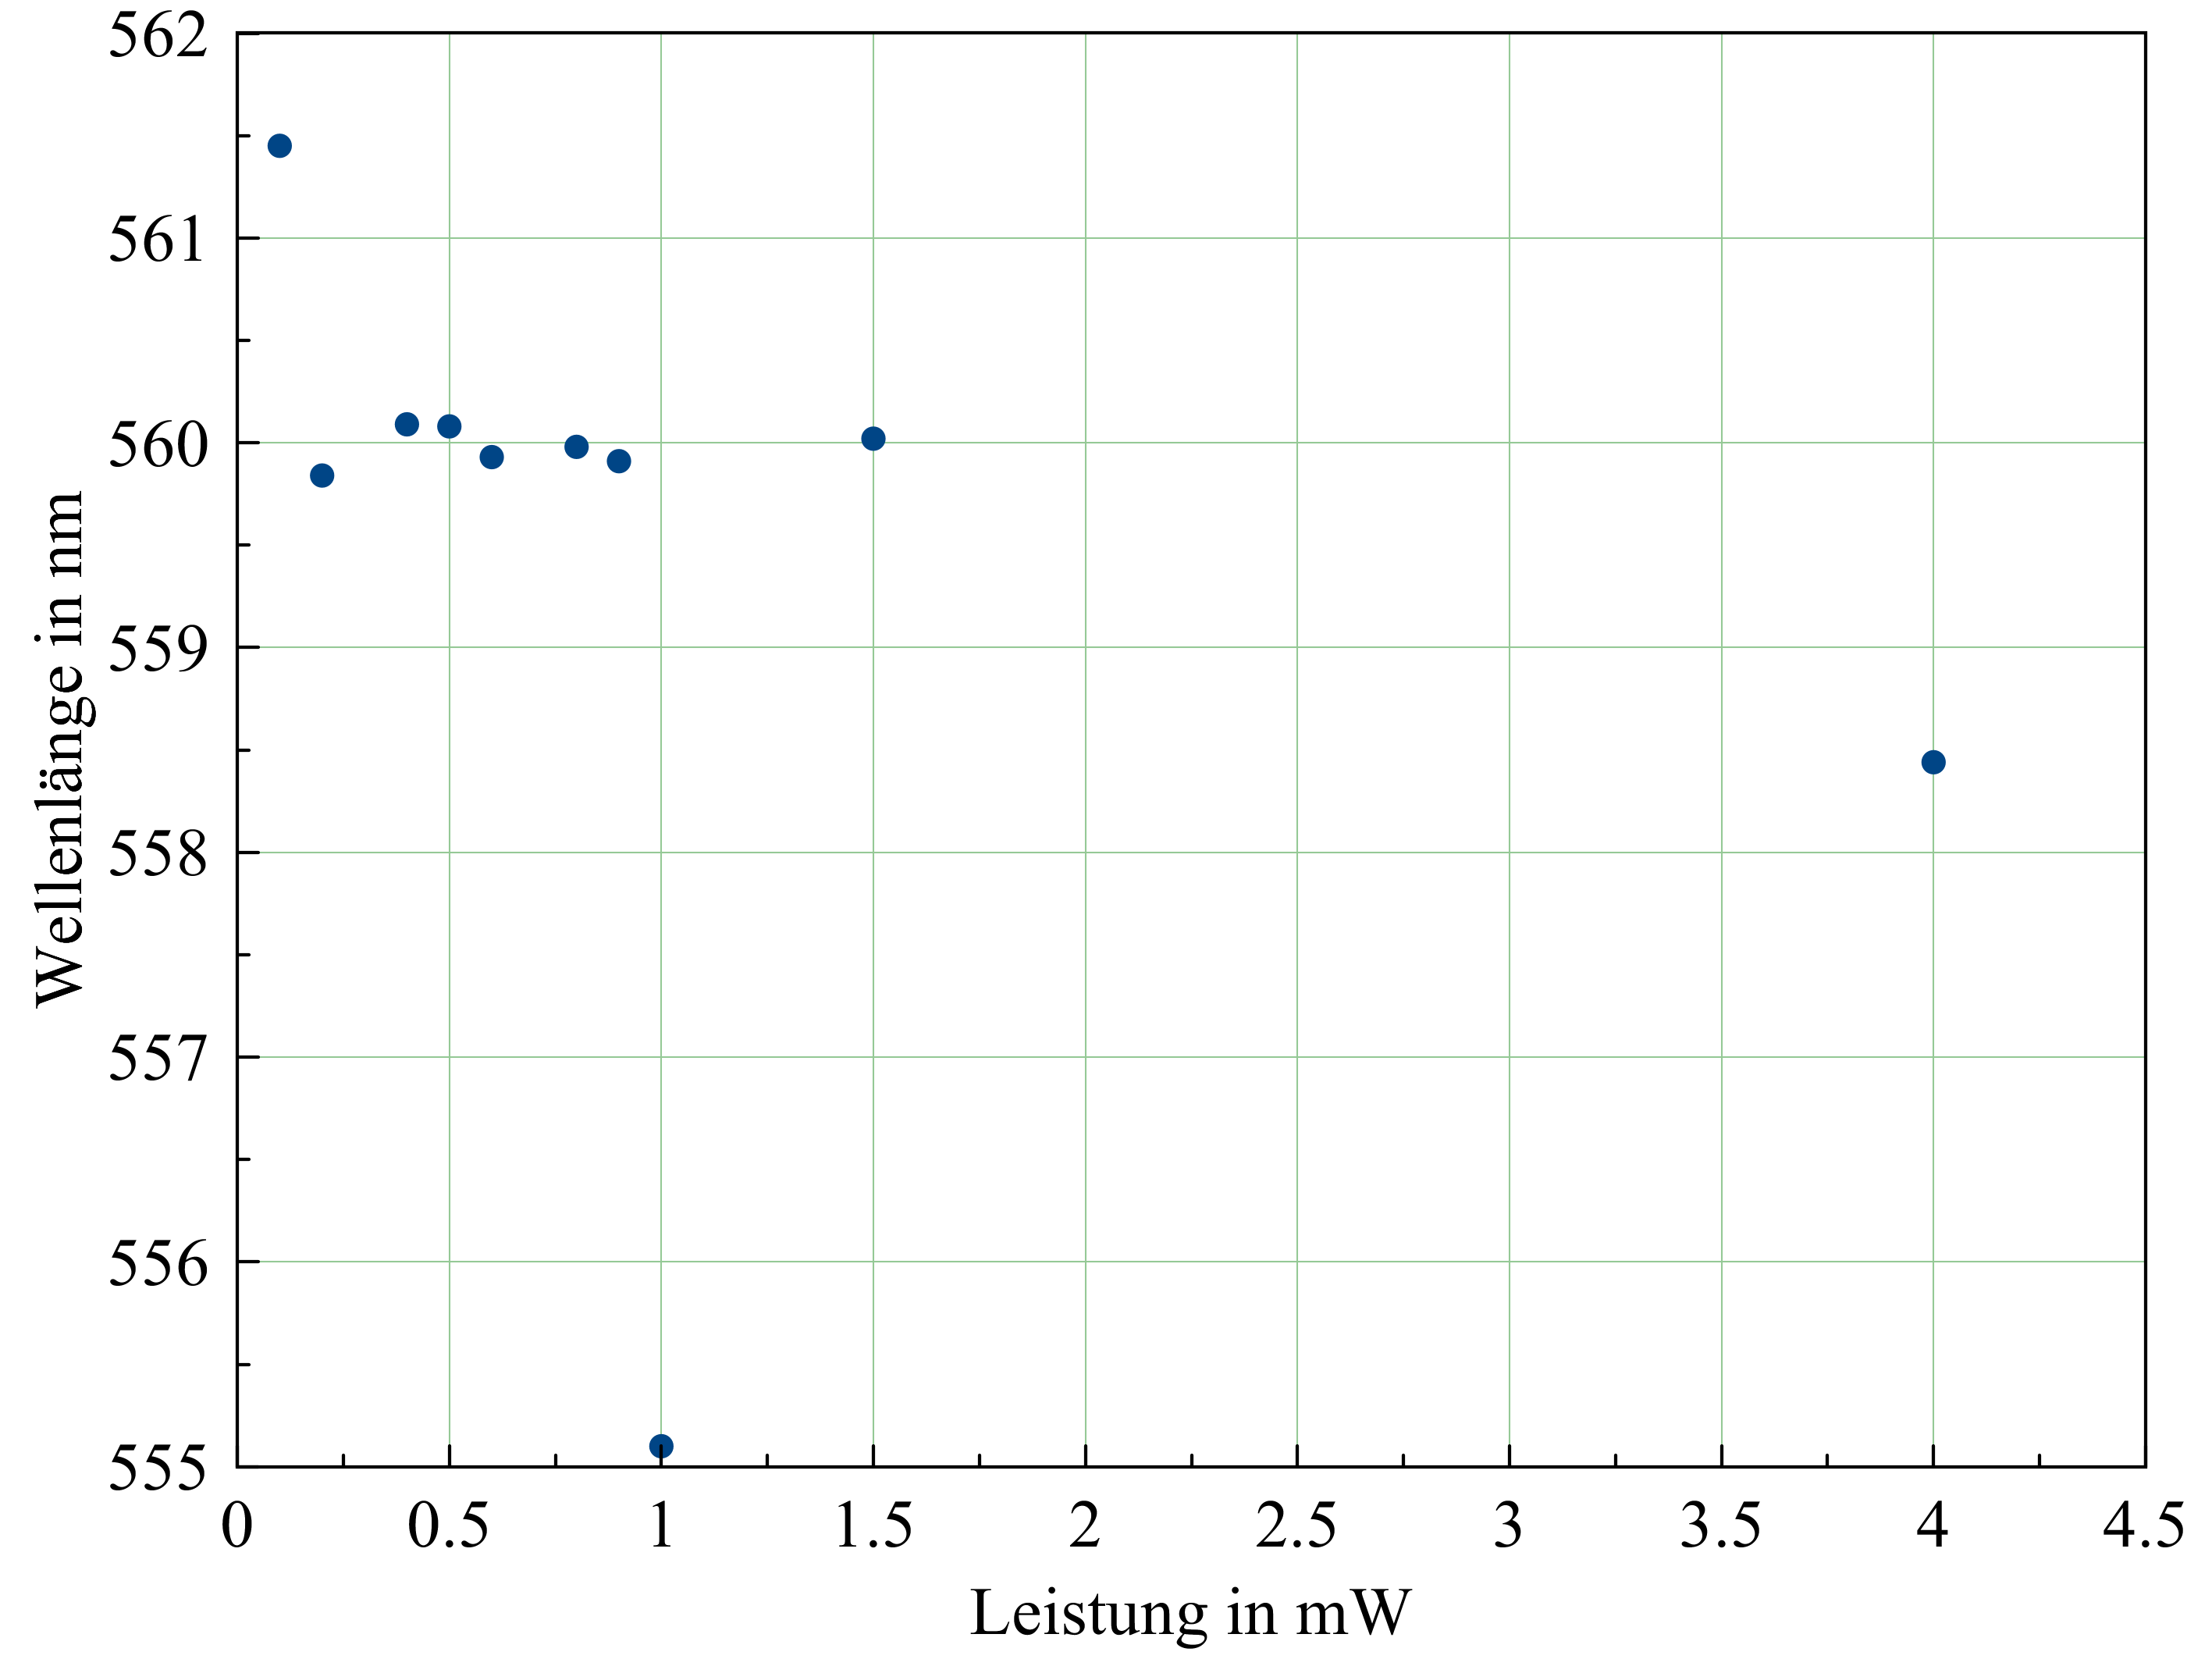
\includegraphics[width=\textwidth]{plots/posemplot_520.png}
    \caption{$\lambda_{\text{pl}} = \SI{520}{\nano\meter}$}
  \end{subfigure}
  \caption{Abhängigkeit der Position des Emissionsmaximums von der Eingangsleistung.}
  \label{fig:posem}
\end{figure}

In den Abbildungen \ref{fig:Podep520} und ~\ref{fig:Podep645} ist außerdem ein Änderung der Halbwertsbreiten der Emissionspeaks mit steigender Leistung erkennbar. Der Zusammenhang von Eingangsleistung und Halbwertsbreite der Emissionspeaks ist daher in Abbildung \ref{fig:FWHM} explizit dargestellt.

\begin{figure}[H]
  \centering
    \begin{subfigure}{0.49\textwidth}
      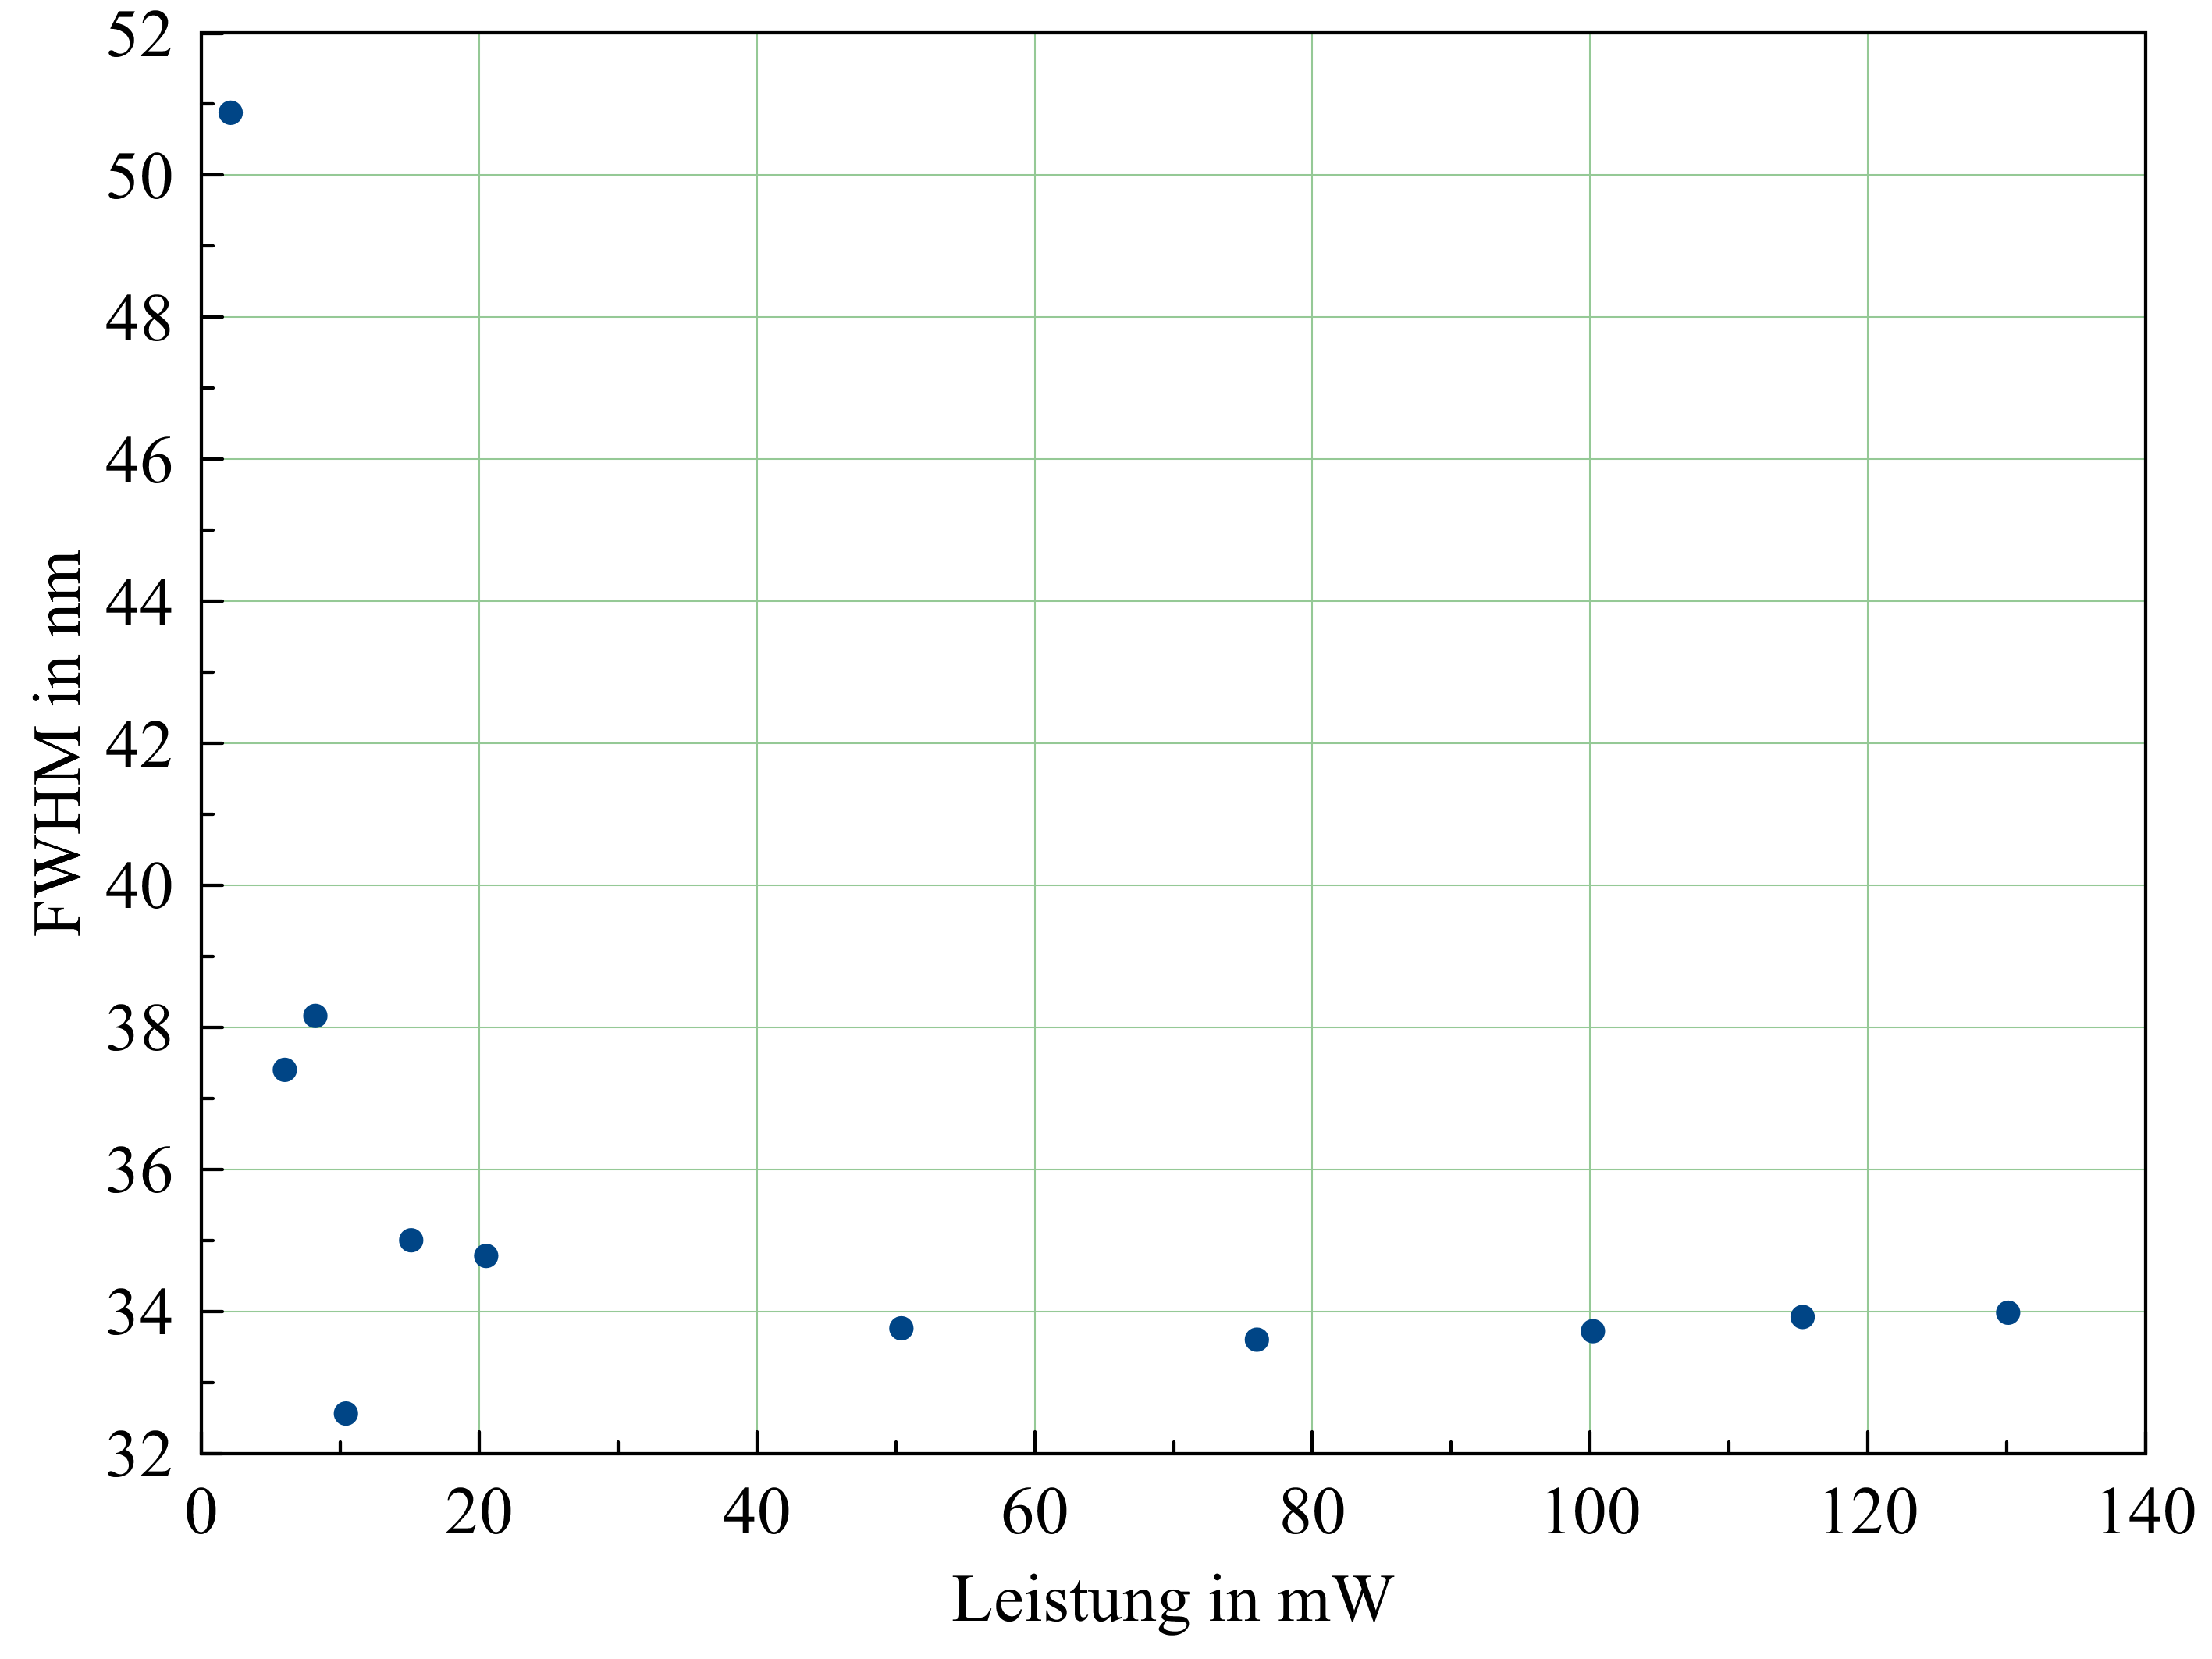
\includegraphics[width=\textwidth]{plots/FWHMplot_645.png}
      \caption{$\lambda_{\text{pl}} = \SI{645}{\nano\meter}$}
    \end{subfigure}
    \begin{subfigure}{0.49\textwidth}
      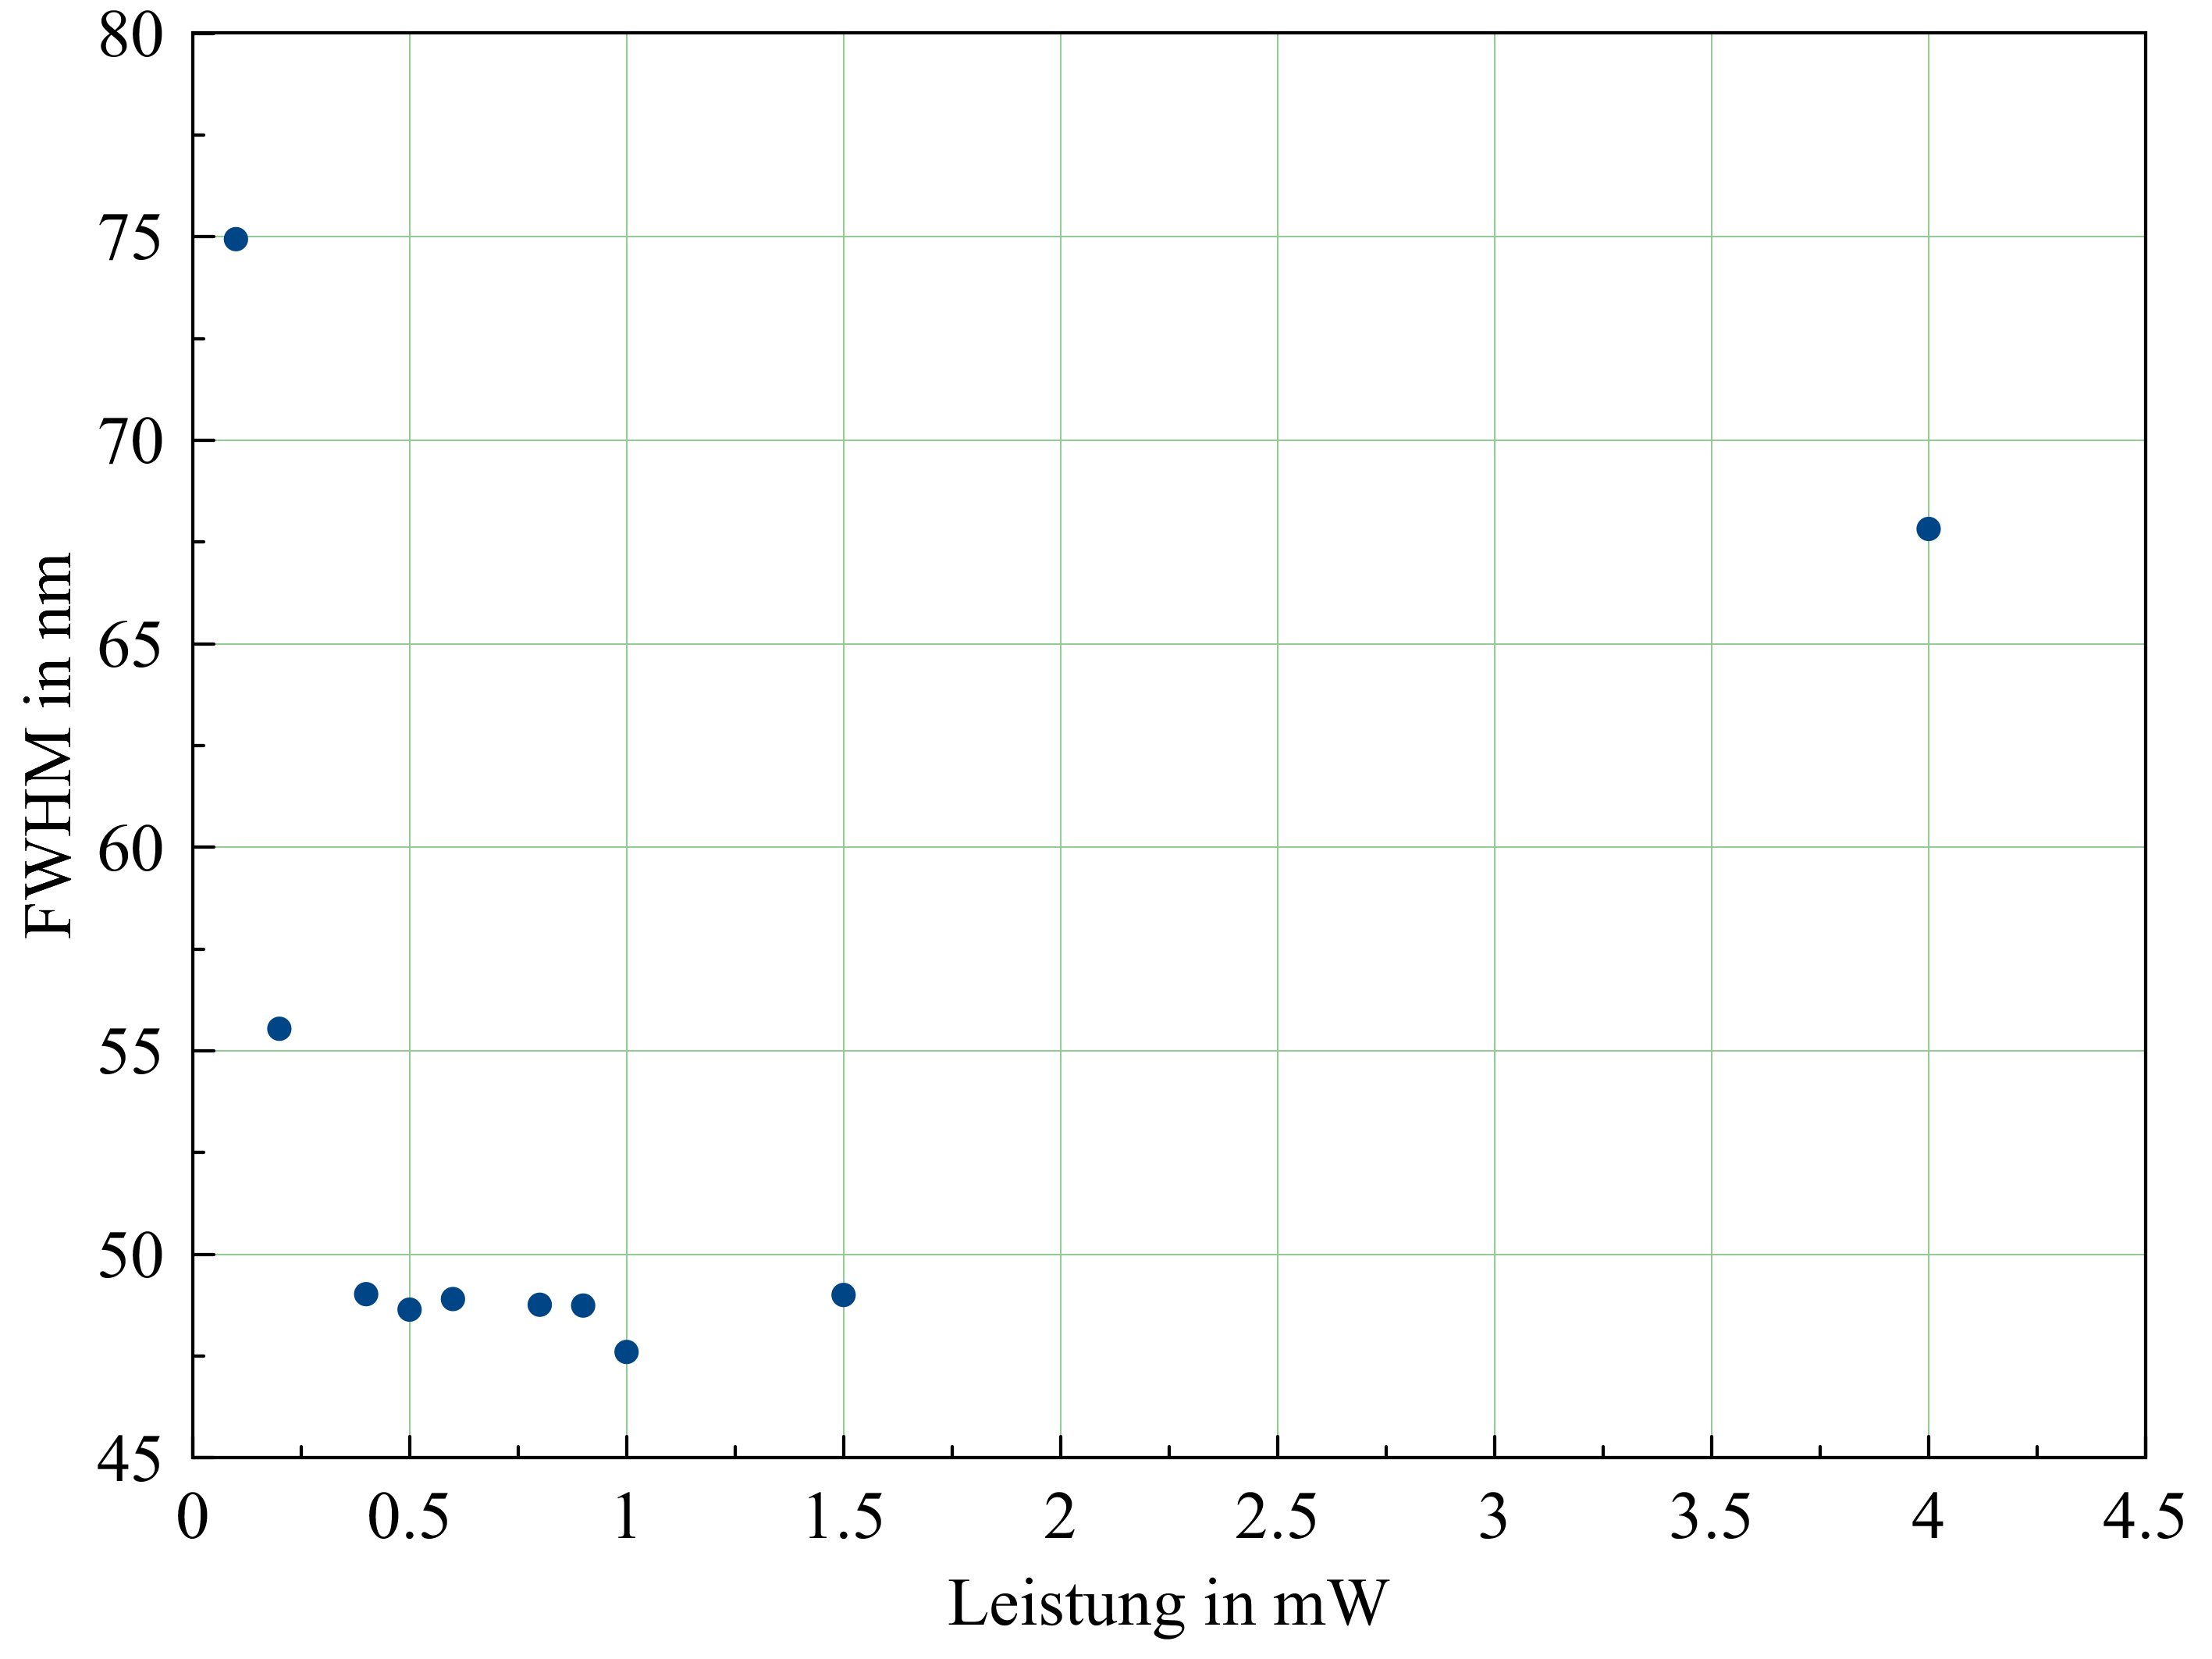
\includegraphics[width=\textwidth]{plots/FWHMplot_520.png}
      \caption{$\lambda_{\text{pl}} = \SI{520}{\nano\meter}$}
    \end{subfigure}
  \caption{Abhängigkeit der Halbwertsbreiten (FWHM) von der Eingangsleistung.}
  \label{fig:FWHM}
\end{figure}
Für kleine Eingangsleistungen ergeben sich bei der $\lambda_{\text{pl}}=\SI{645}{\nano\meter}$ Probe hohe Halbwertsbreiten, welche mit zunehmender Leistung schnell kleiner werden und sich dann einem konstanten Wert annähern. Die Halbwertsbreiten der $\lambda_{\text{pl}}=\SI{520}{\nano\meter}$ Probe zeigen bis auf den bei $\SI{4}{\milli\watt}$ aufgenommenen Messwert ähnliches Verhalten.

\subsection{Abhängigkeit der PL von der Polarisation}
\label{sec:Polarisation}
Um eine Abhängigkeit von der Polarisation des eingestrahlten Lichtes festzustellen wurden für drei verschiedene lineare Polarisationen Photolumineszenzspektren einer Probe aufgenommen. Anregungswellenlänge und  Eingangsleistung wurden hier nicht verändert. Aus den gemessenen Spektren (Abbildung \ref{fig:Polarisation}) geht hervor, dass die Photolumineszenz nicht von der Polarisation des anregenden Lichtes abhängt.
\begin{figure}[H]
  \centering
  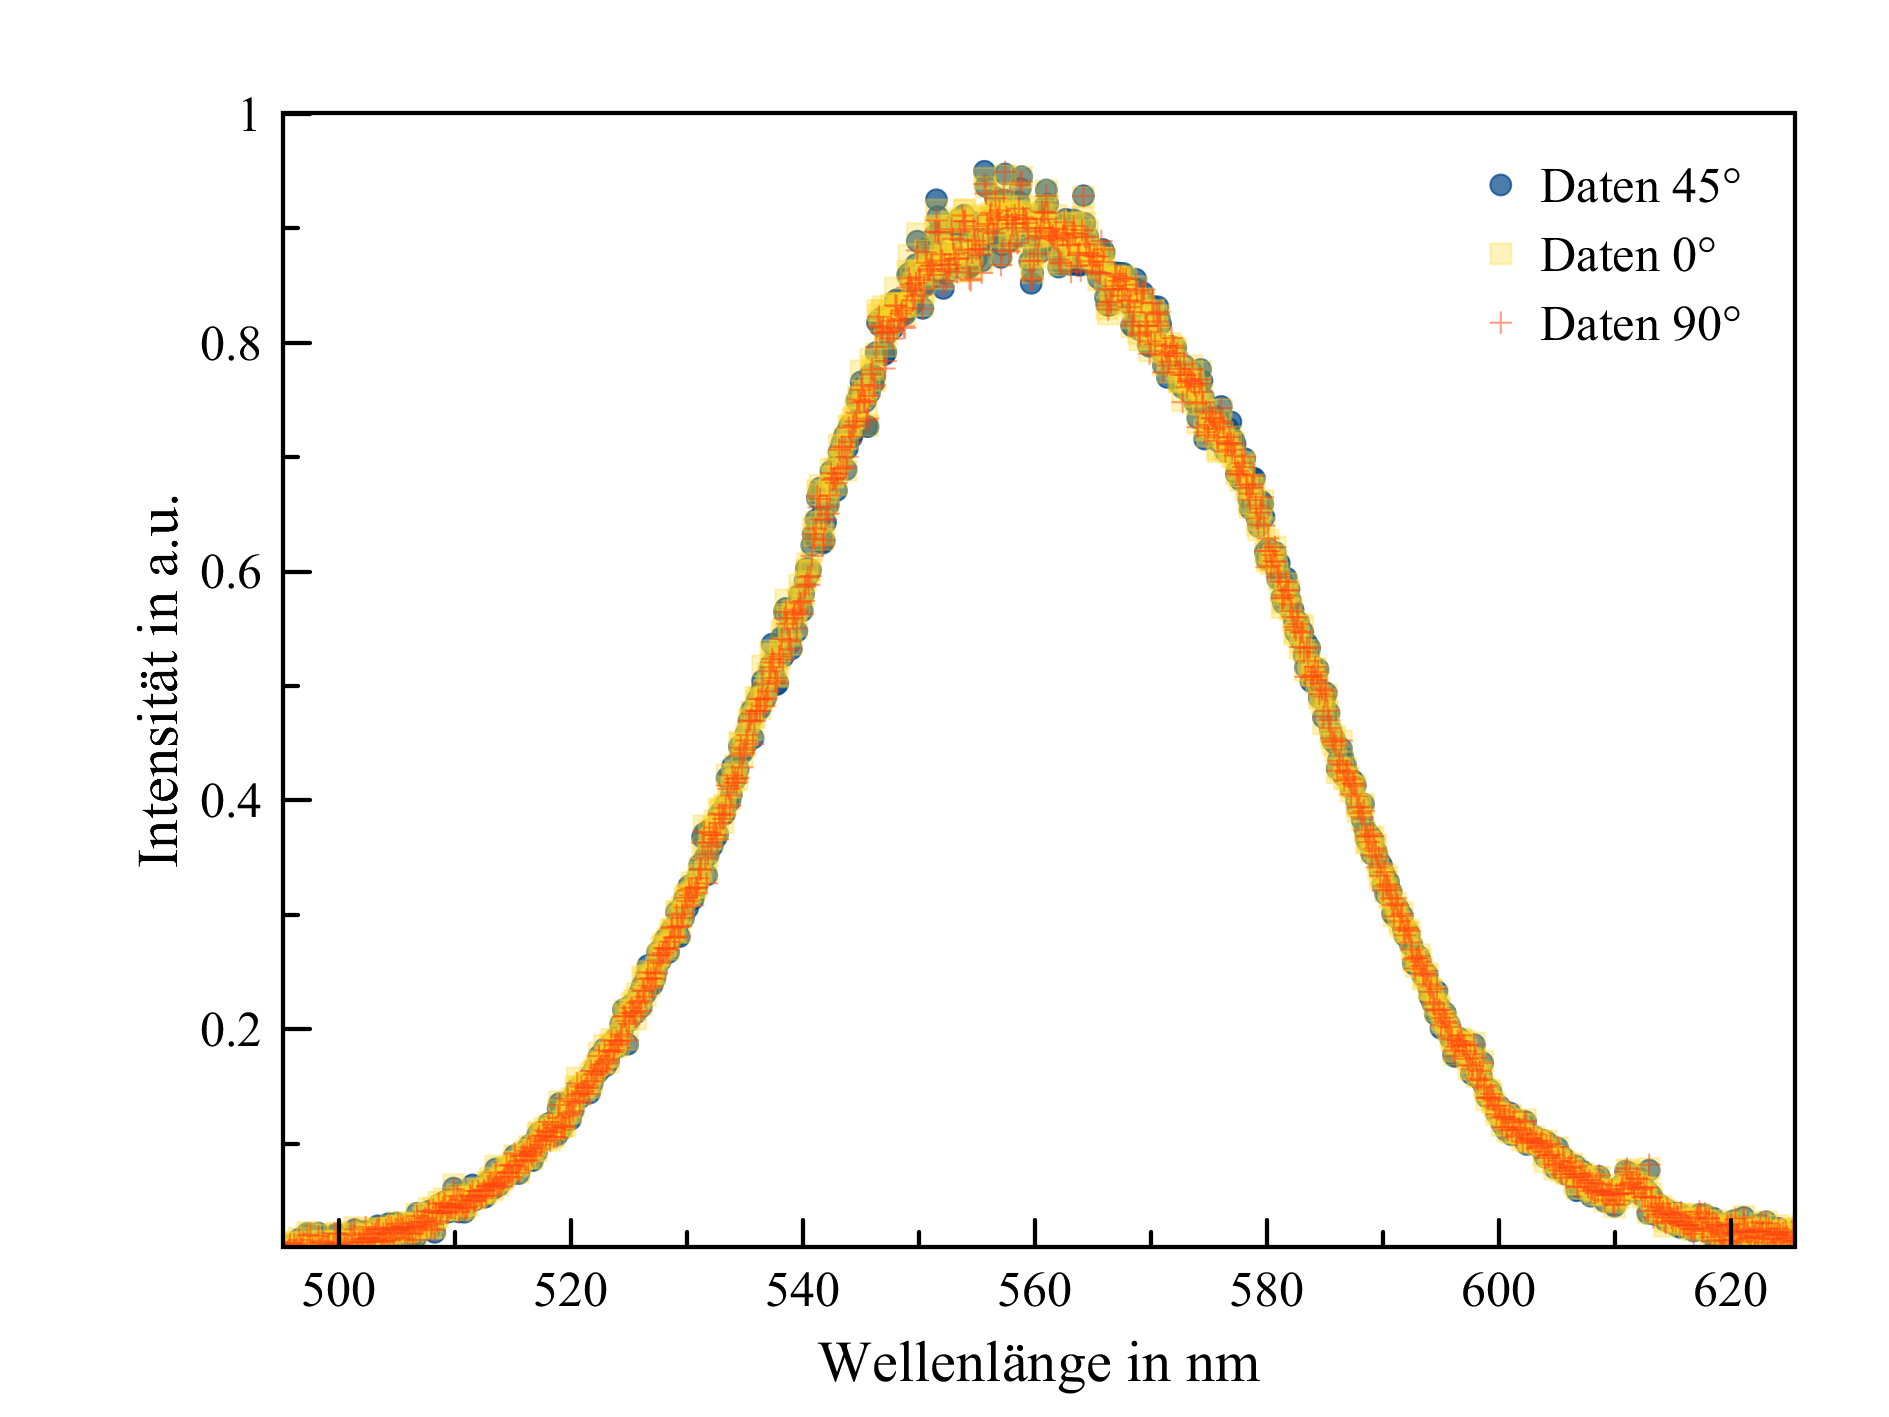
\includegraphics[width=0.7\textwidth]{plots/Poldepplot.png}
  \caption{Abhängigkeit der Photolumineszenz der $\lambda_{\text{PL}}=\SI{520}{\nano\meter}$
   Probe bei einer Anregungswellenlänge von $\lambda=\SI{405}{\nano\meter}$ und einer Eingangsleistung von $\SI{1,5}{\milli\watt}$.}
   \label{fig:Polarisation}
\end{figure}

\subsection{Photolumineszenz bei anderen Anregungsenergien}
\label{sec:weisslicht}
Zuletzt wurden Photolumineszentspektren aller drei Proben für zwei weitere Anregungswellenlängen, $\SI{520}{\nano\meter}$ und $\SI{470}{nm}$ aufgenommen. Die Ergebnisse sind in den Abbildungen \ref{fig:PL_645} bis \ref{fig:PL_520} dargestellt. In Abbildung \ref{fig:PL_580_Satt} ist die Sättigung der Photodiode deutlich zu sehen. Für die $\lambda_{\text{pl}}\SI{645}{\nano\meter}$  ist keine Photolumineszenz der Probe auszumachen und es ist nur die Reflexion der Anregung zusehen. In den weiteren Spektren ist diese Reflexion klar von dem, durch die Photolumineszenz entstehenden Peak, unterscheidbar. Es fällt auf, dass die Photolumineszenz eine deutlich höhere spektrale Breite aufweist, als die spektrale Breite der Anregung.
\begin{figure}[H]
  \centering
  \begin{subfigure}{0.49\textwidth}
    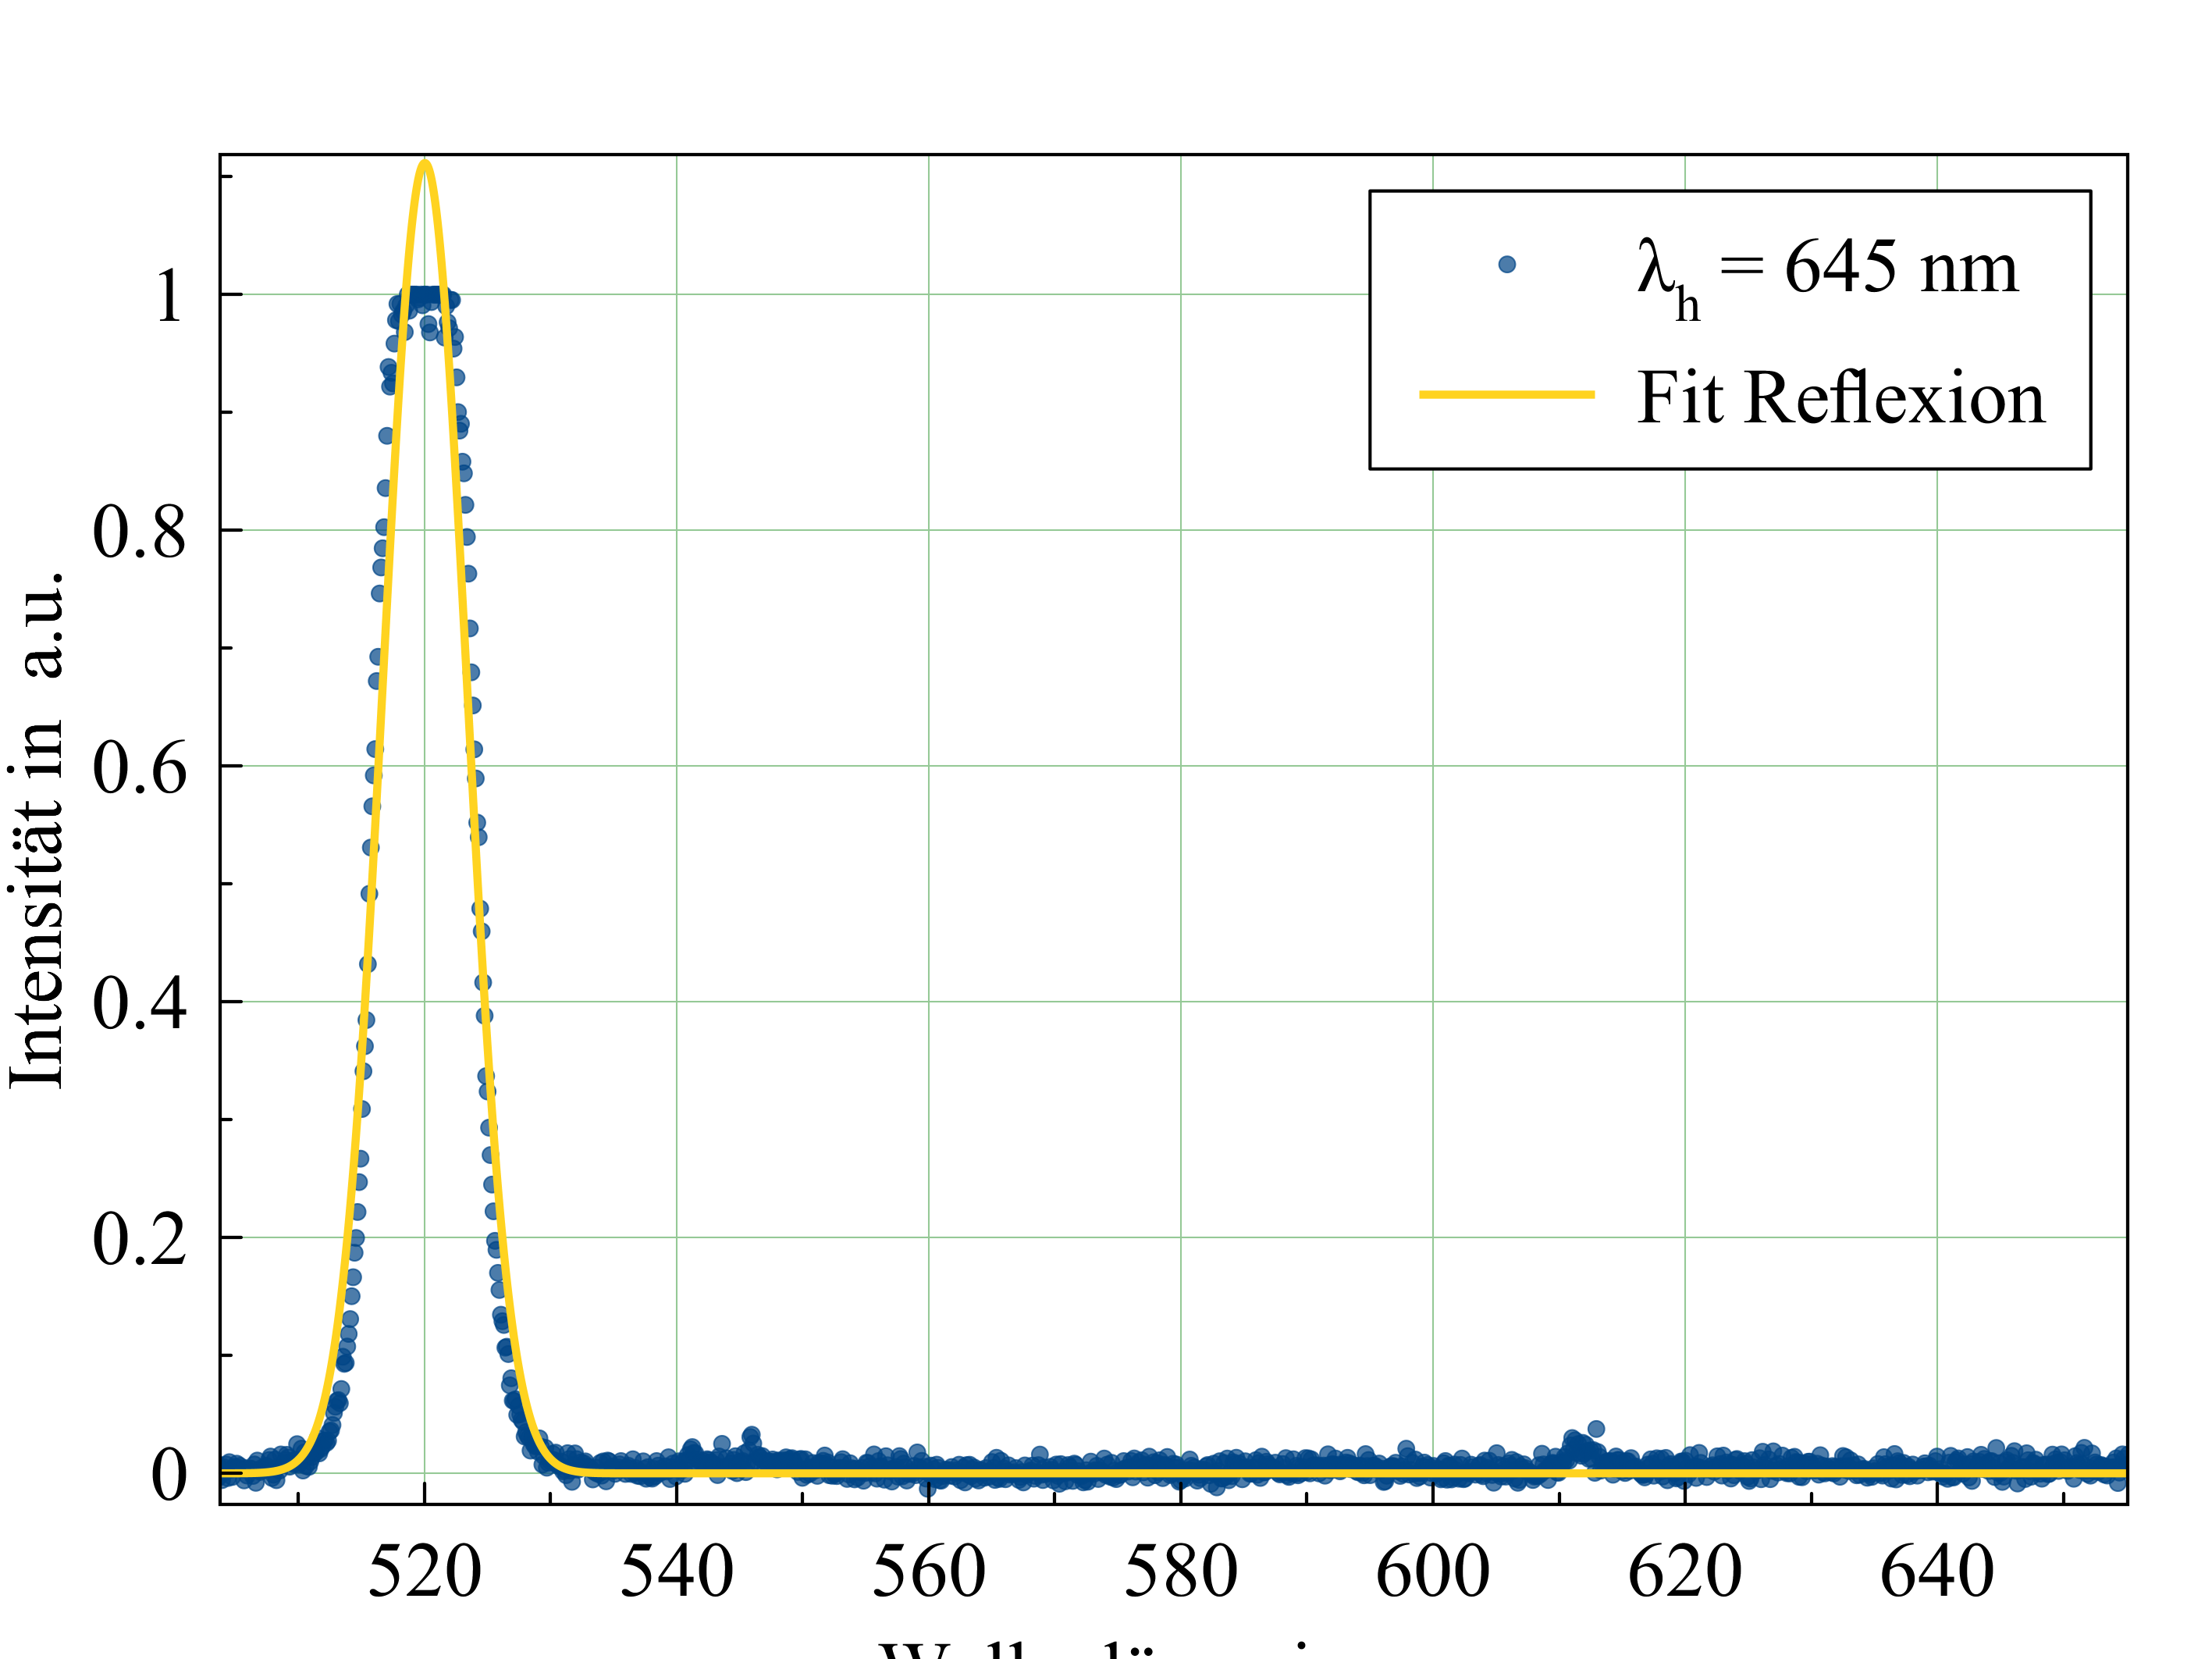
\includegraphics[width=\textwidth]{plots/Weisslicht_645_520.png}
    \caption{$\lambda=\SI{520}{\nano\meter}$}
  \end{subfigure}
  \begin{subfigure}{0.49\textwidth}
    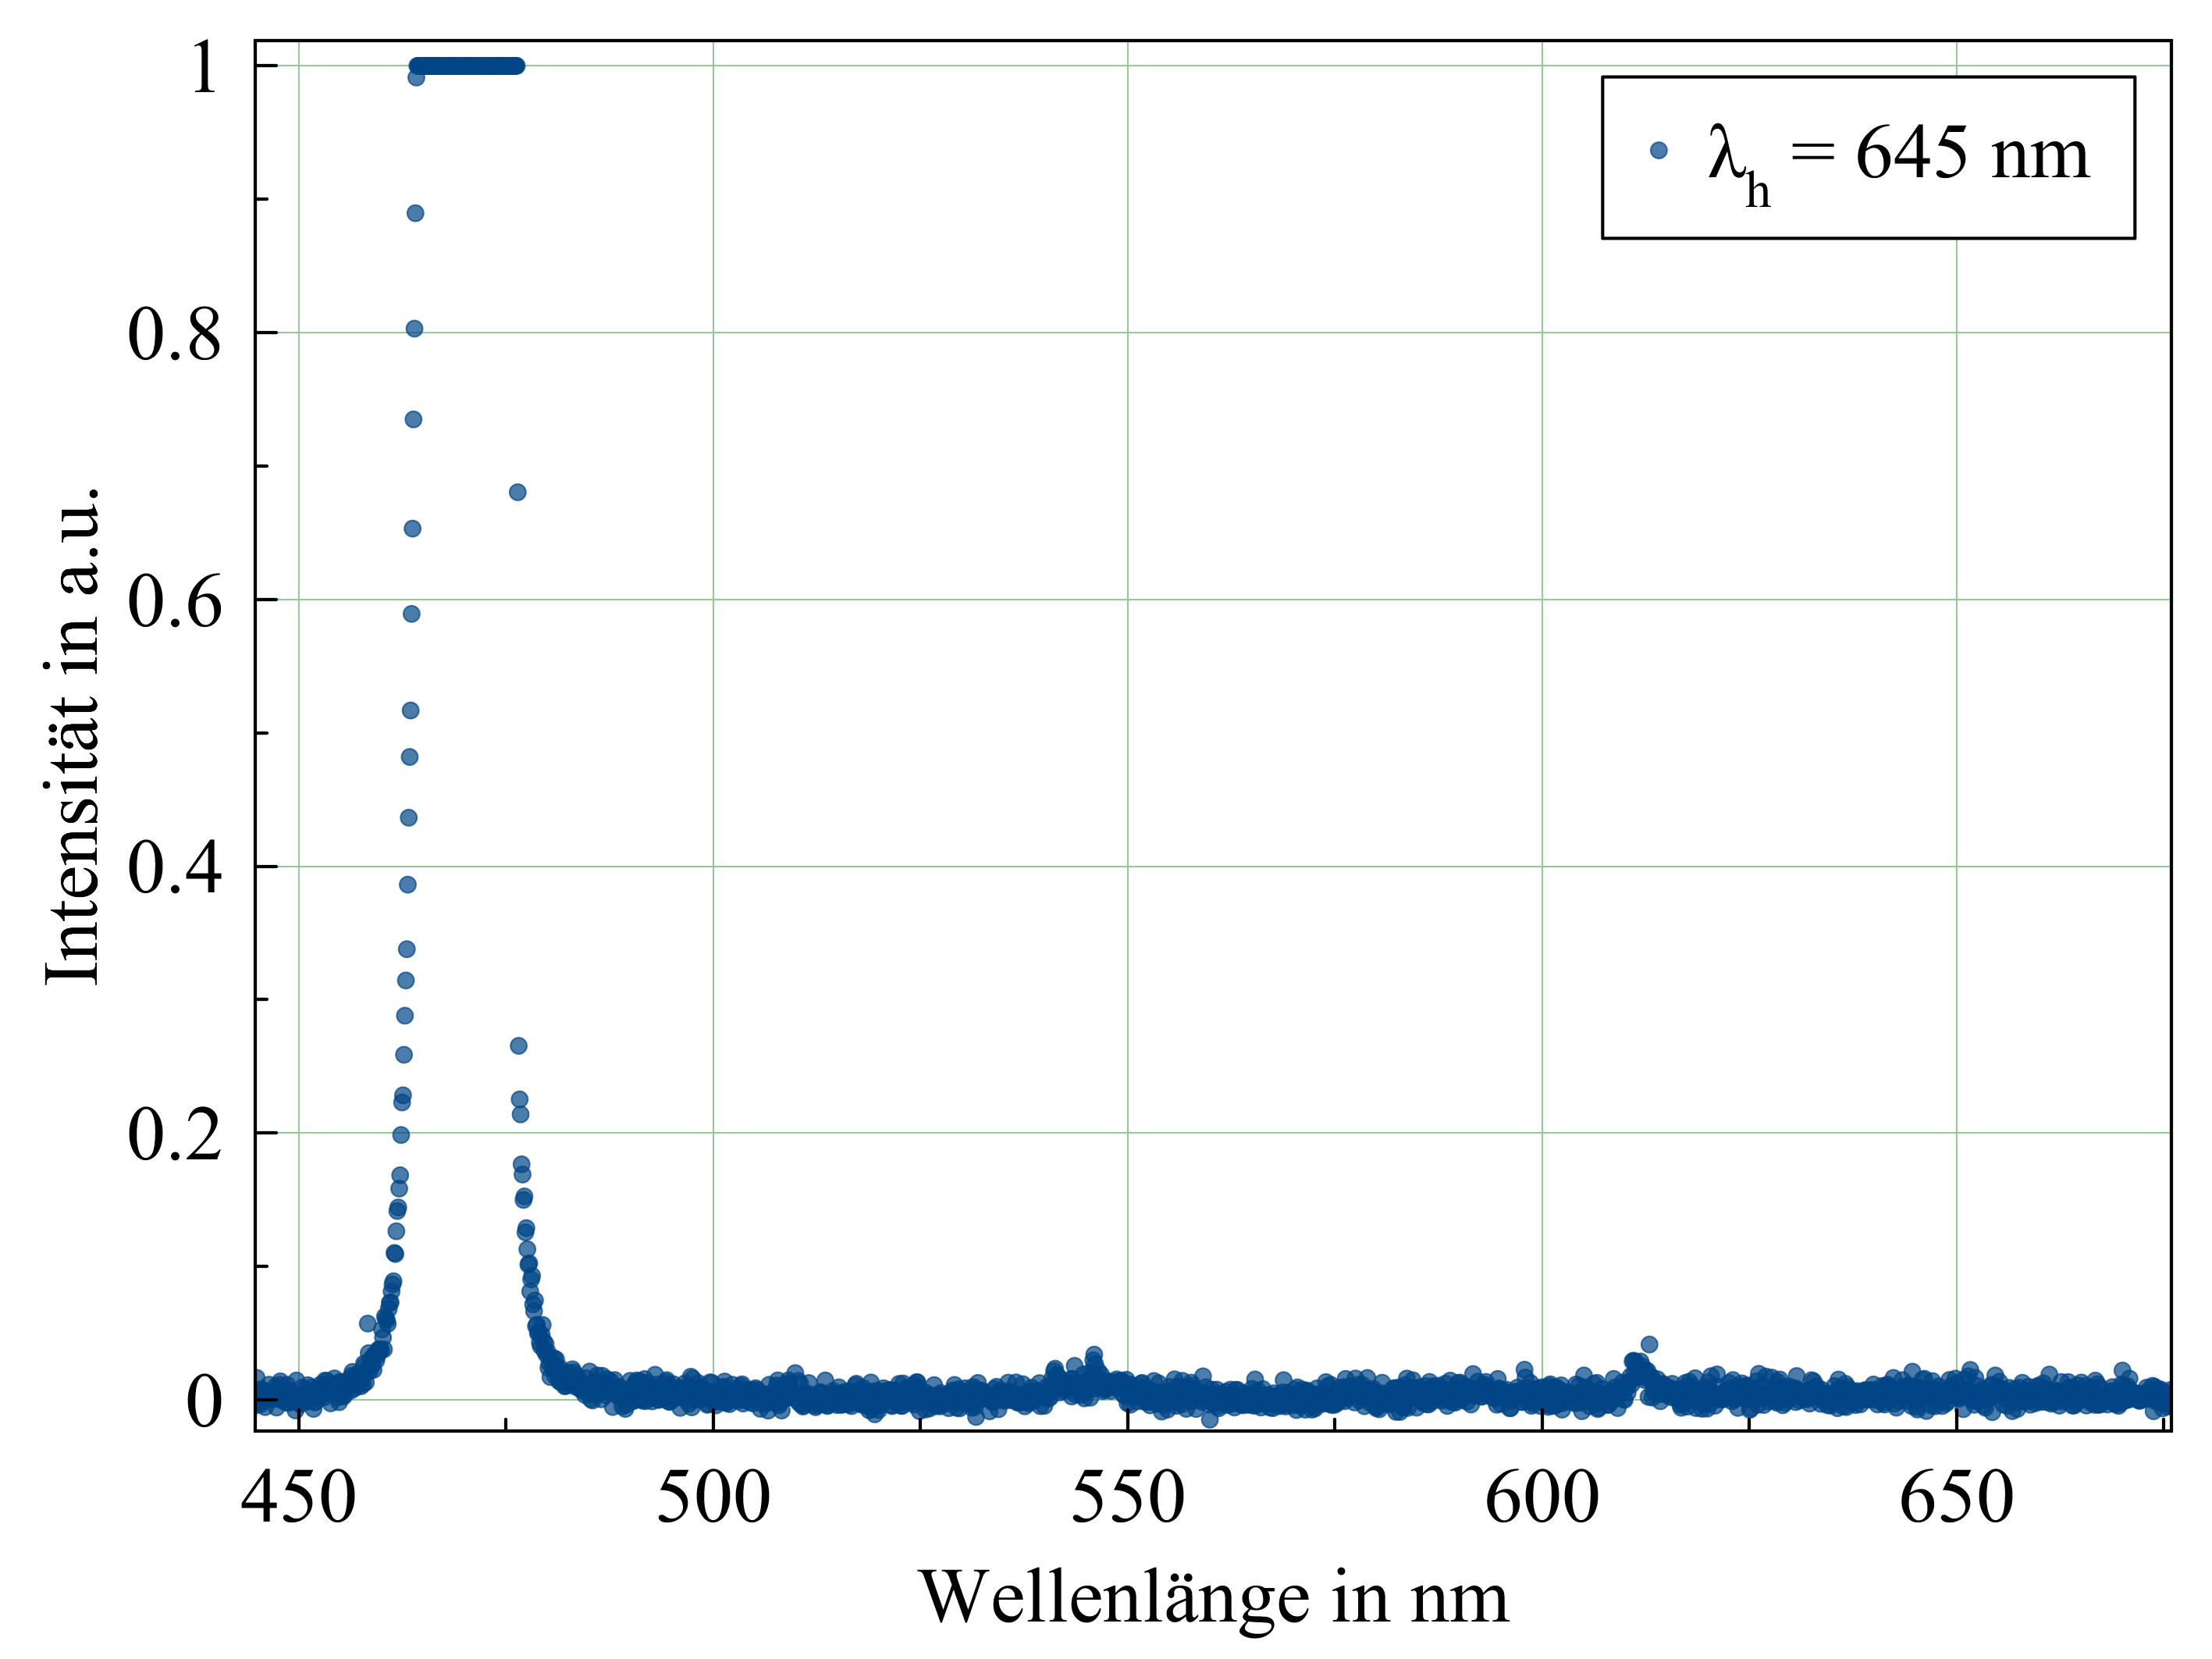
\includegraphics[width=\textwidth]{plots/Weisslicht_645_470.png}
    \caption{$\lambda=\SI{470}{\nano\meter}$}
  \end{subfigure}
  \caption{Photolumineszenzspektrum der $\lambda_{\text{PL}}=\SI{645}{\nano\meter}$ Probe.}
  \label{fig:PL_645}
\end{figure}
\begin{figure}[H]
  \centering
  \begin{subfigure}{0.49\textwidth}
    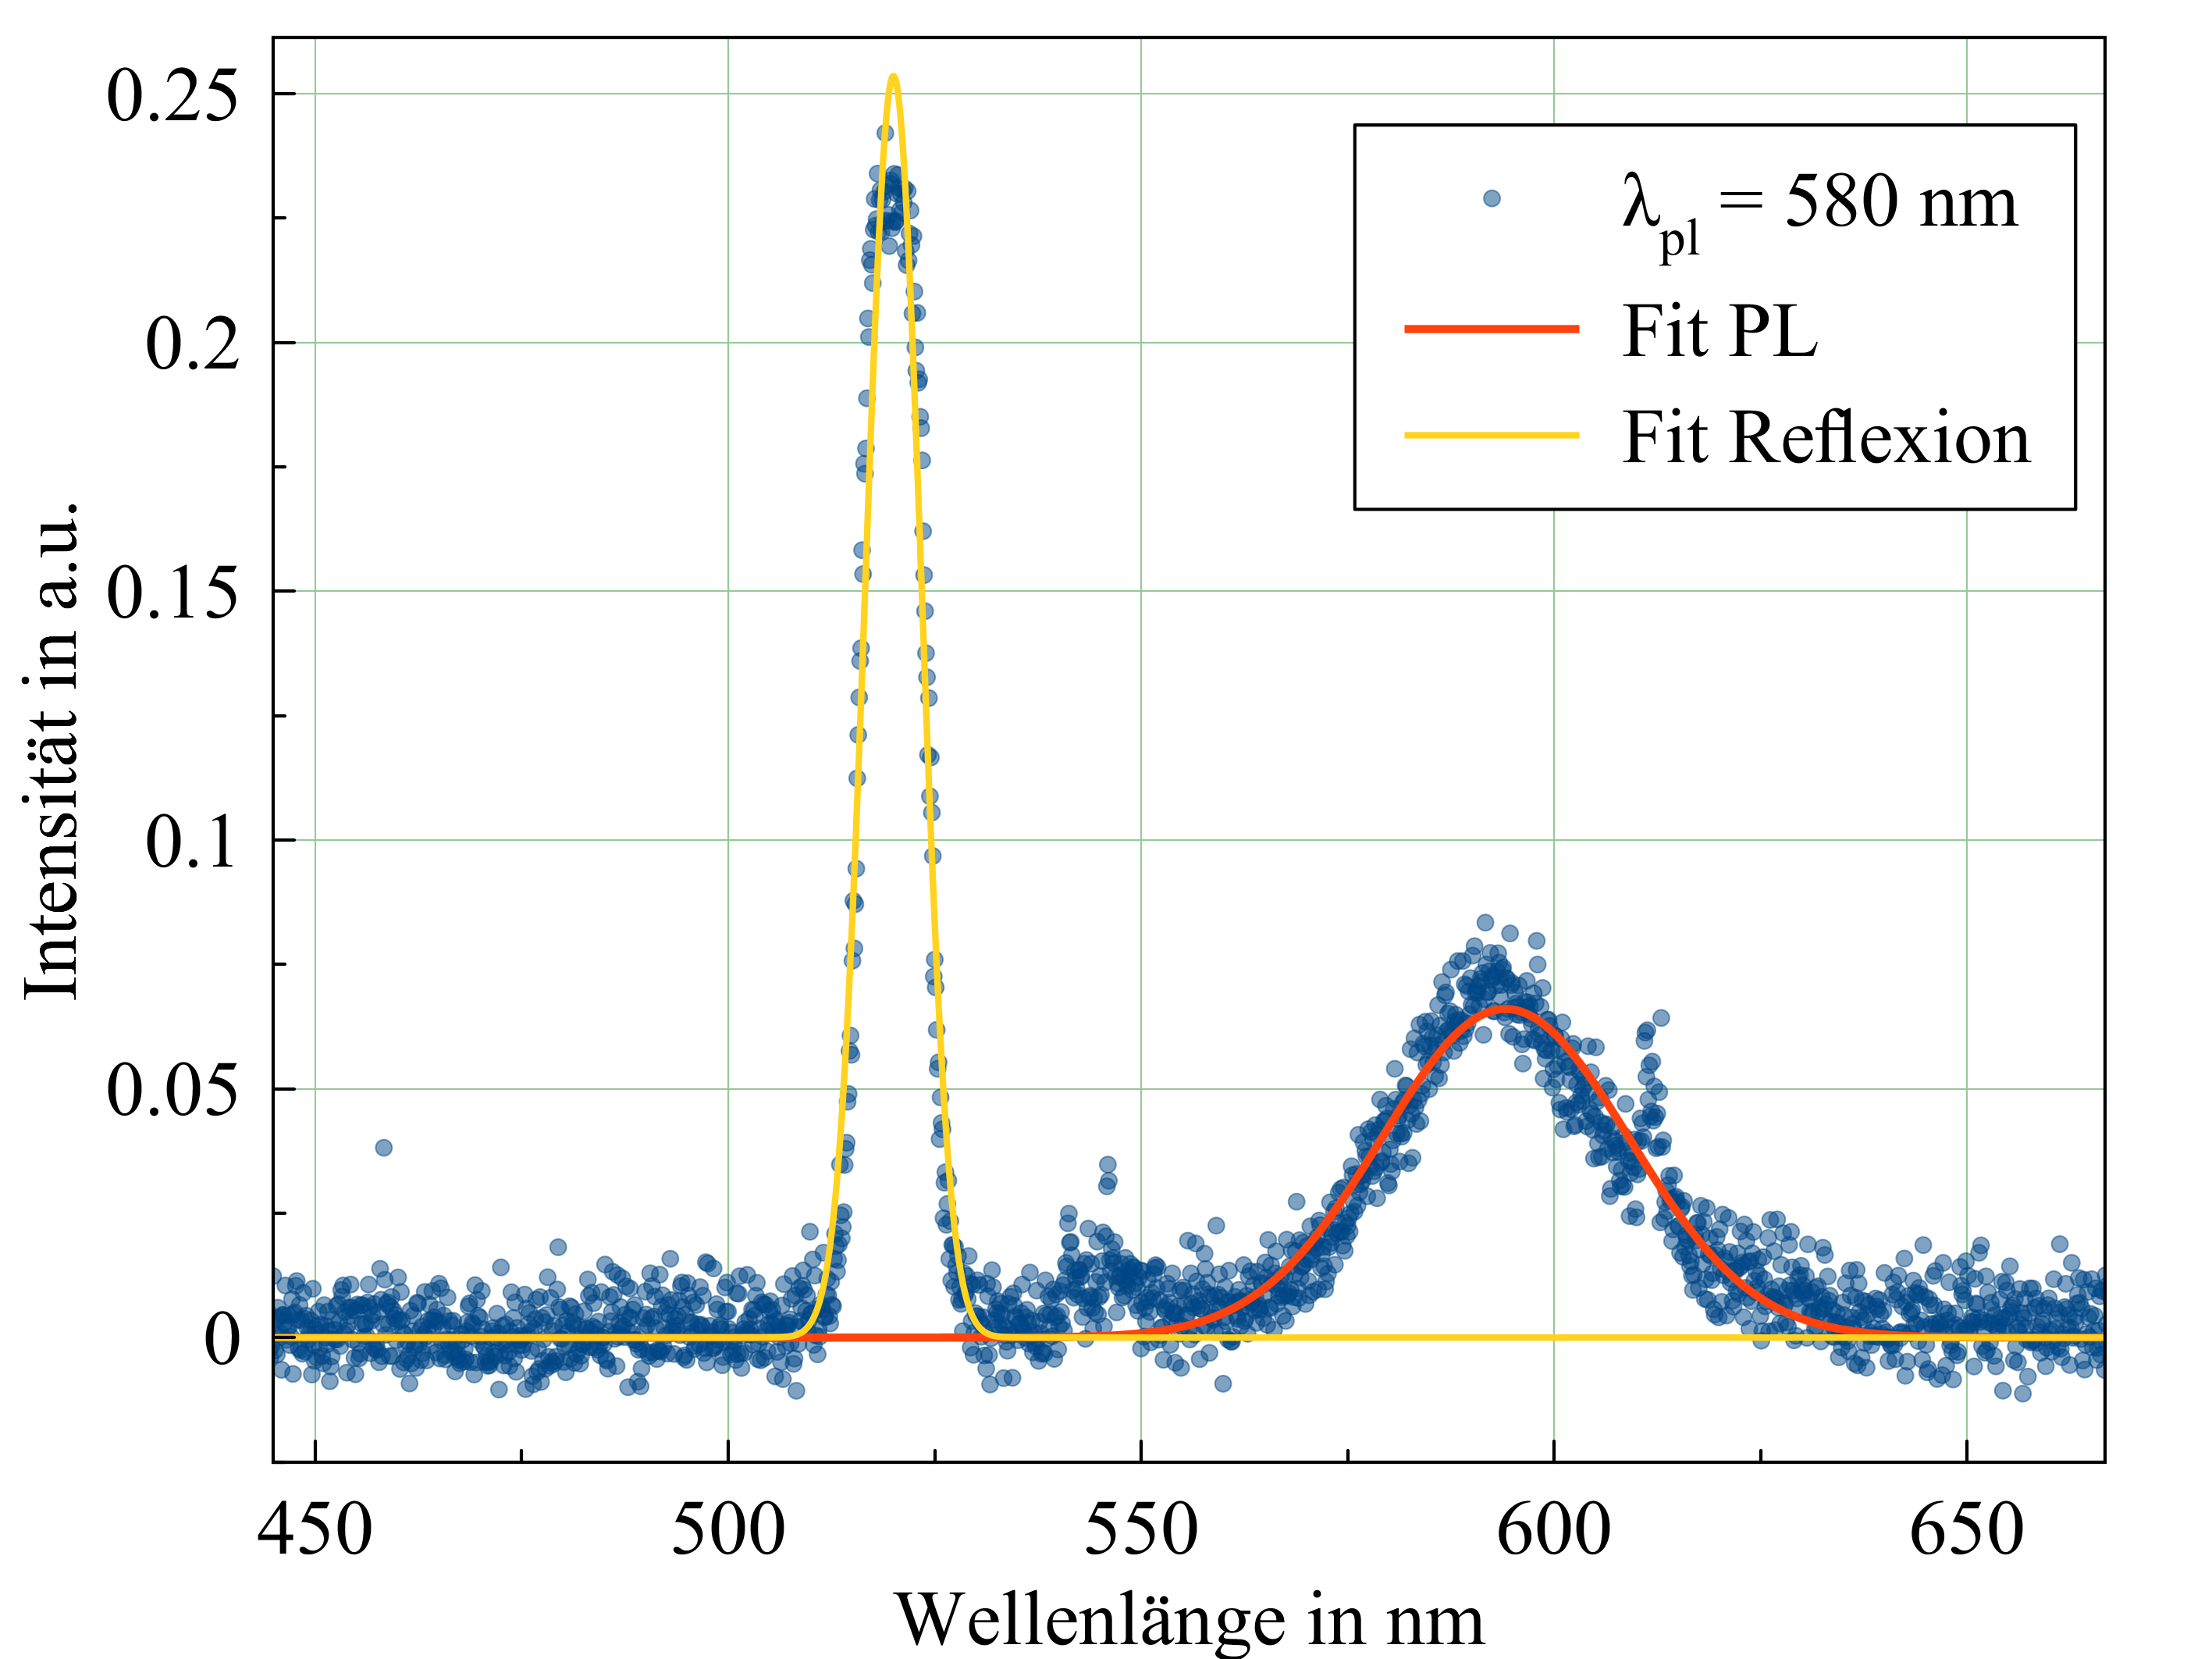
\includegraphics[width=\textwidth]{plots/Weisslicht_580_520.png}
    \caption{$\lambda=\SI{520}{\nano\meter}$}
    \label{fig:PL_580_normus}
  \end{subfigure}
  \begin{subfigure}{0.49\textwidth}
    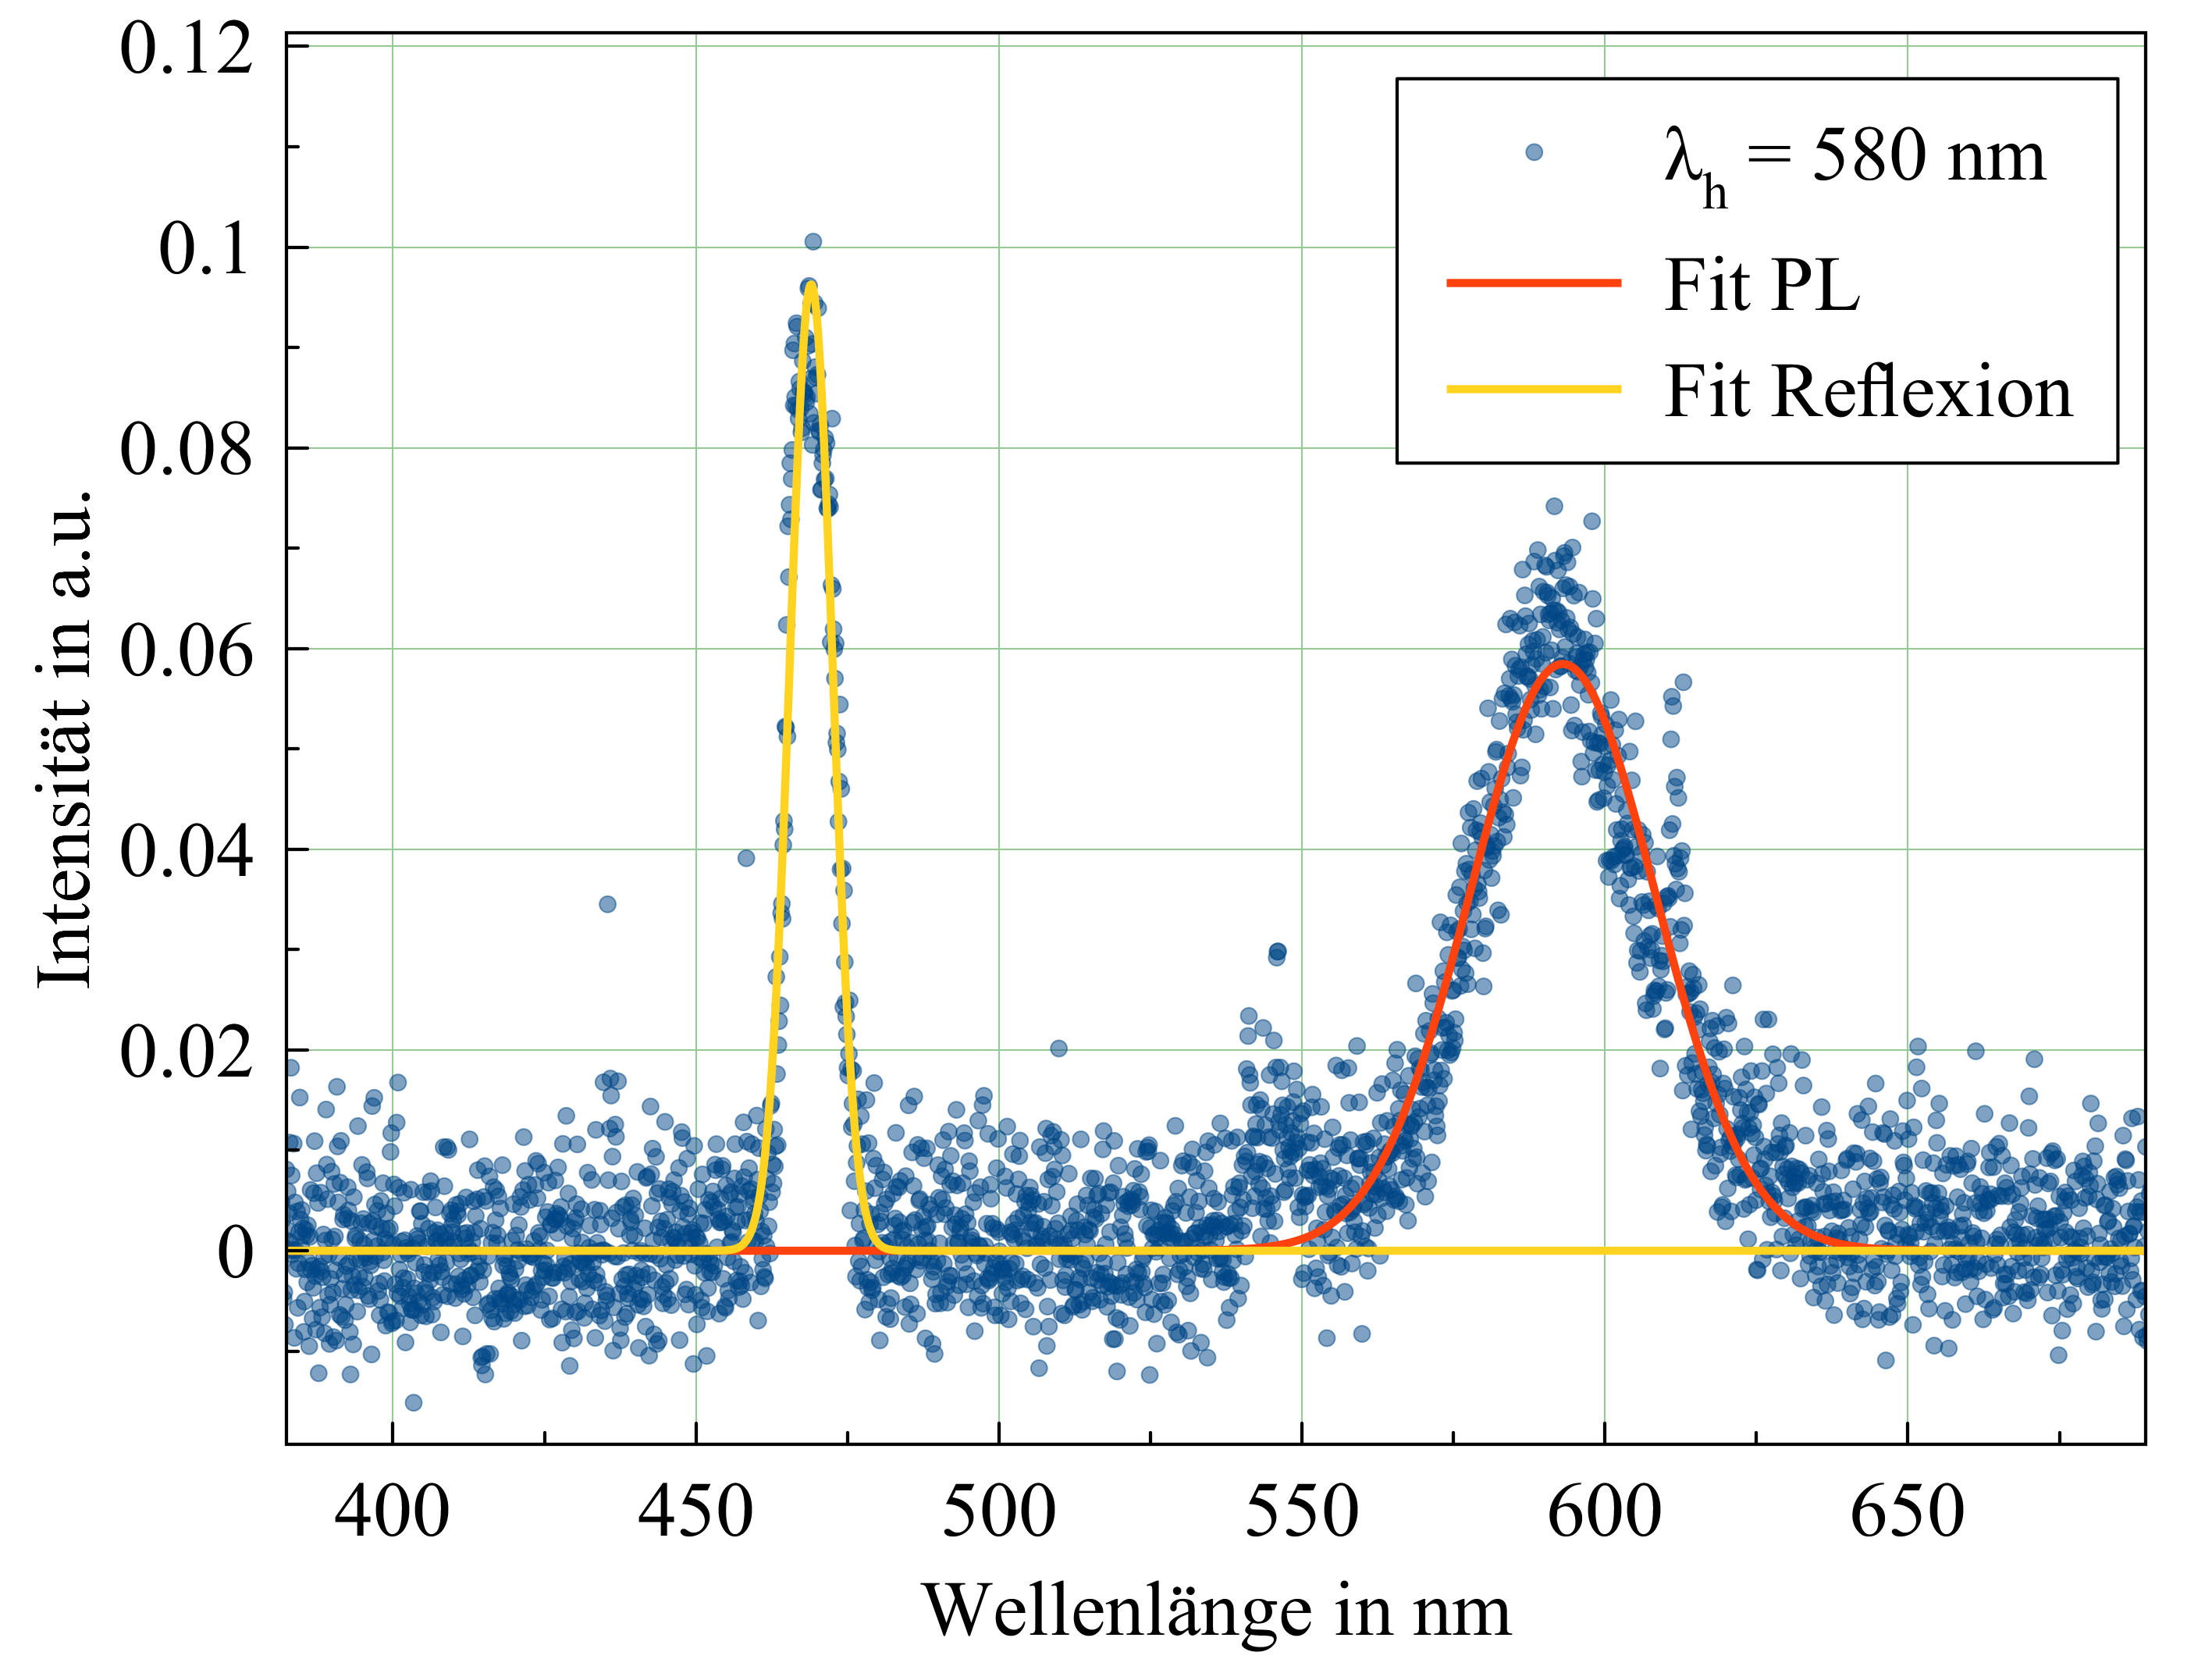
\includegraphics[width=\textwidth]{plots/Weisslicht_580_470.png}
    \caption{$\lambda=\SI{470}{\nano\meter}$}
    \label{fig:PL_580_Satt}
  \end{subfigure}
  \caption{Photolumineszenzspektrum der $\lambda_{\text{PL}}=\SI{580}{\nano\meter}$ Probe.}
  \label{fig:PL_580}
\end{figure}
\begin{figure}[H]
  \centering
  \begin{subfigure}{0.49\textwidth}
    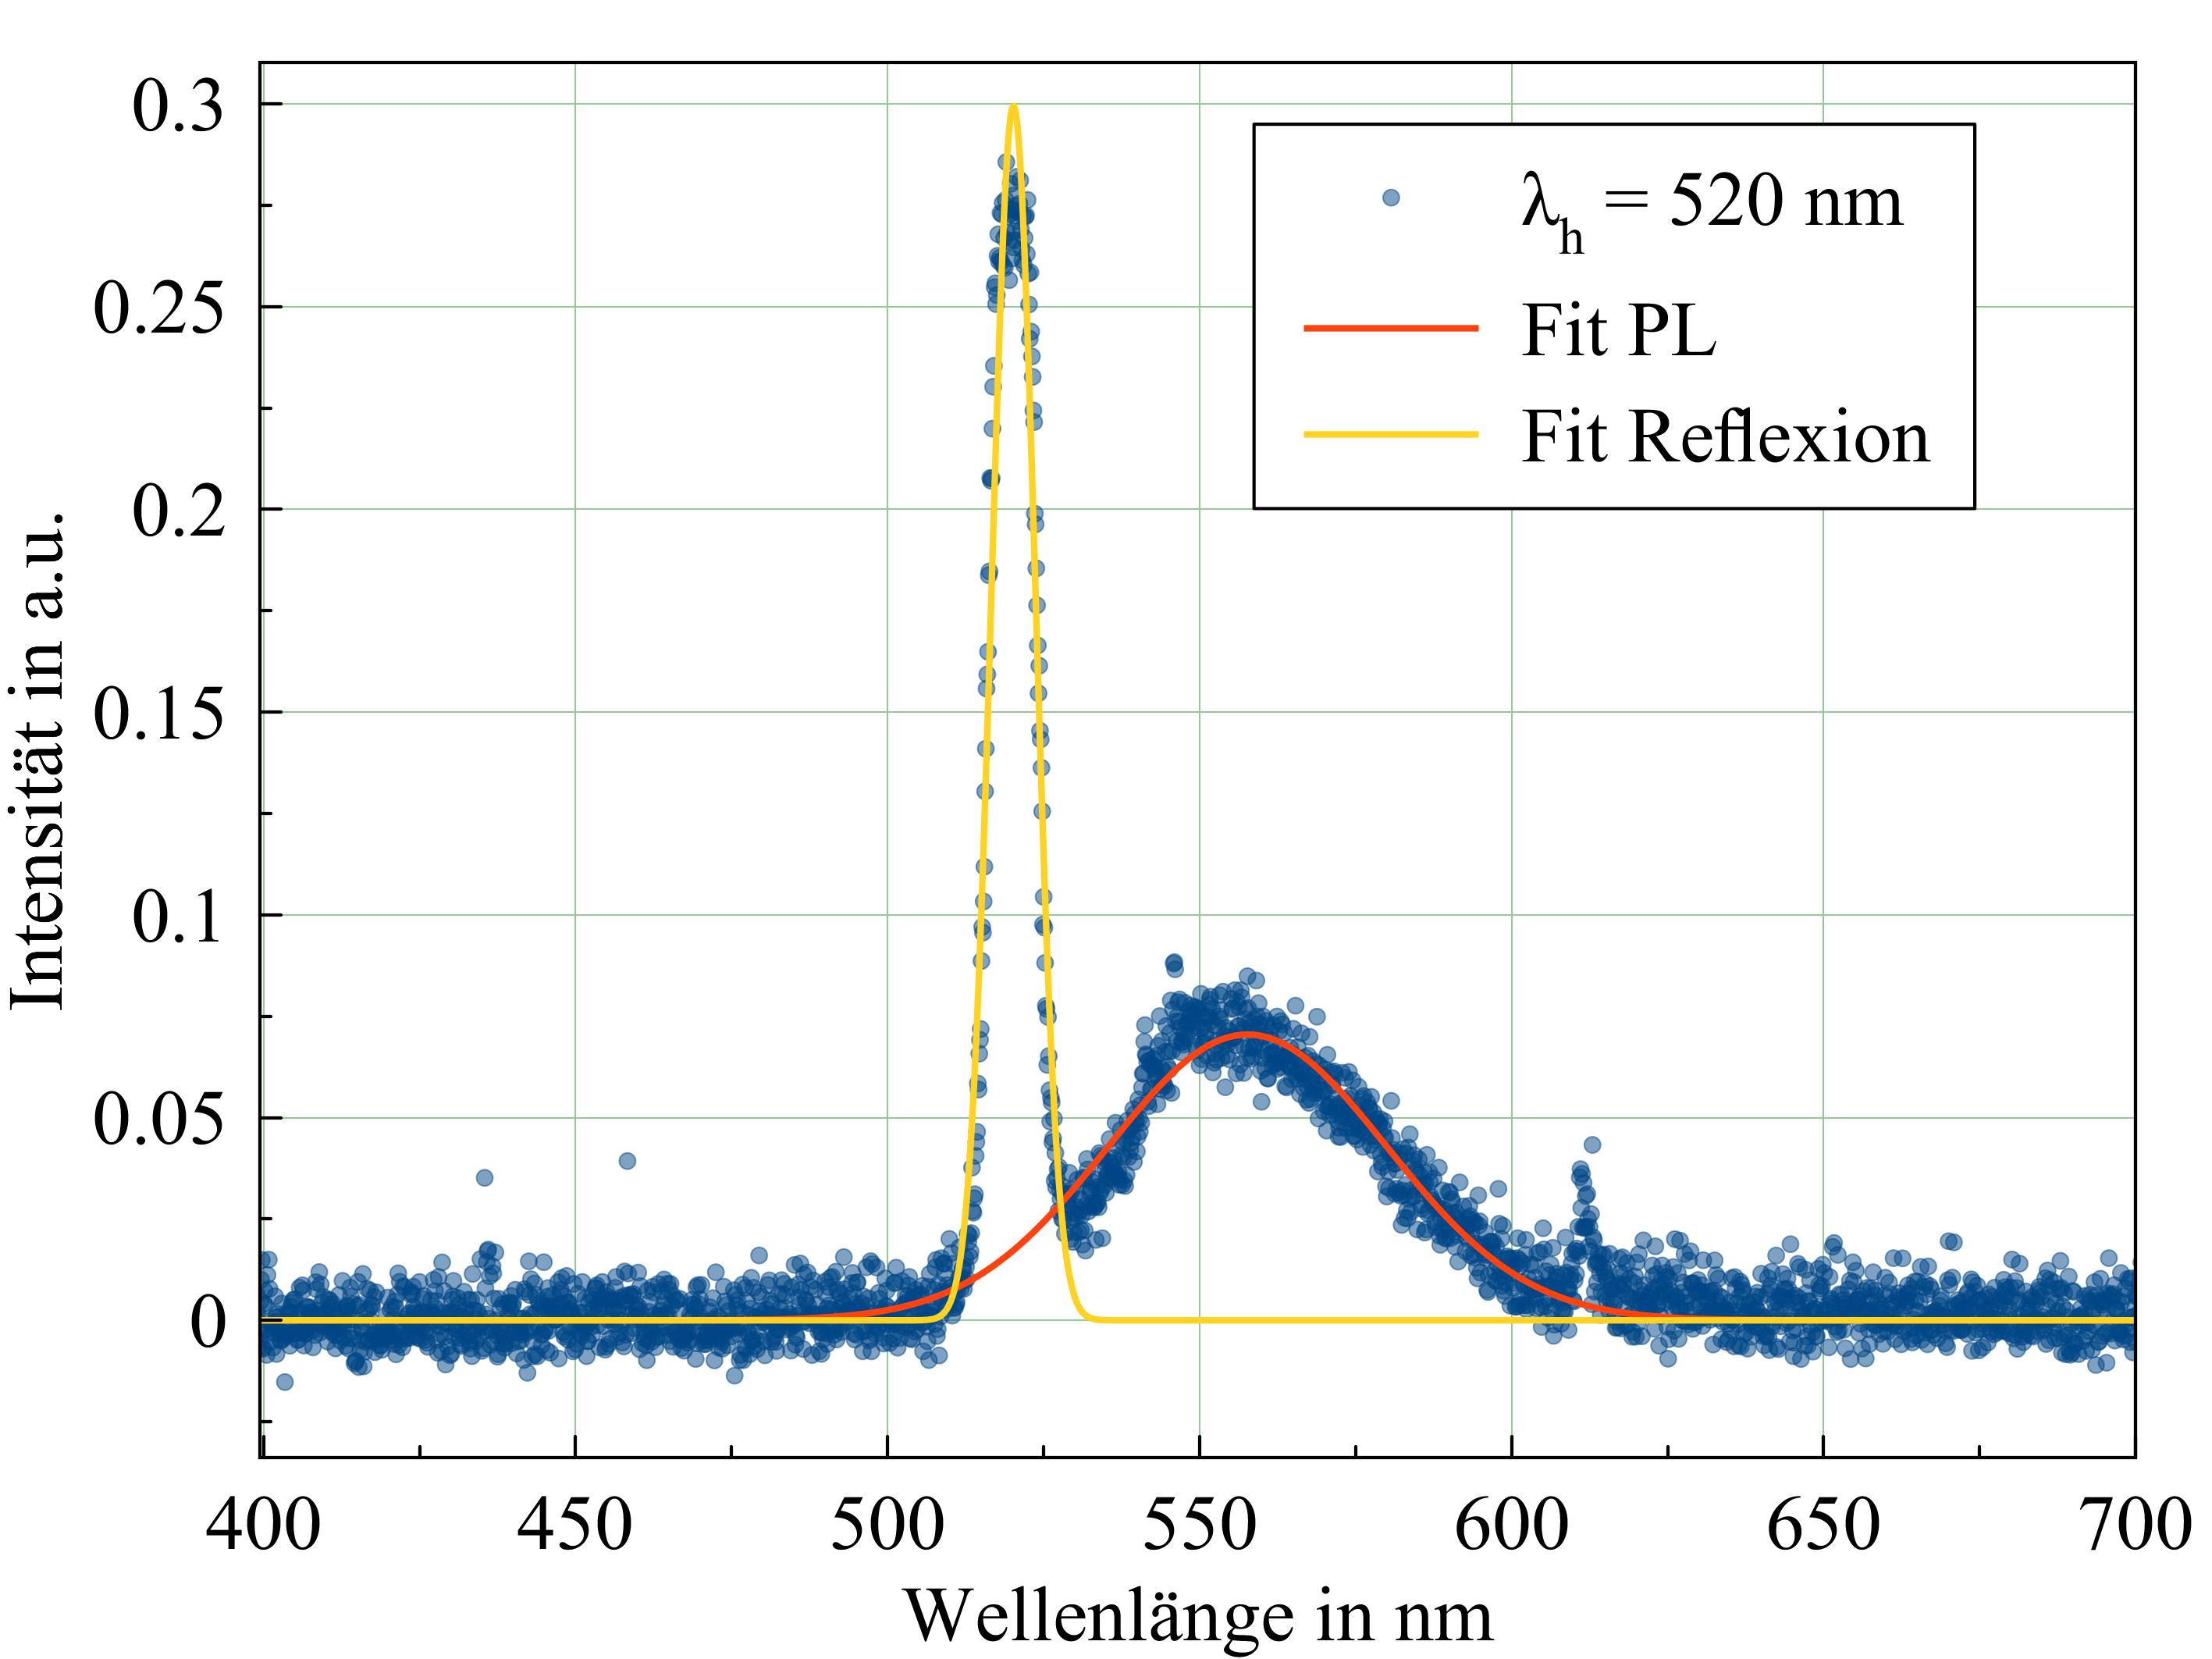
\includegraphics[width=\textwidth]{plots/Weisslicht_520_520.png}
    \caption{$\lambda=\SI{520}{\nano\meter}$}
  \end{subfigure}
  \begin{subfigure}{0.49\textwidth}
    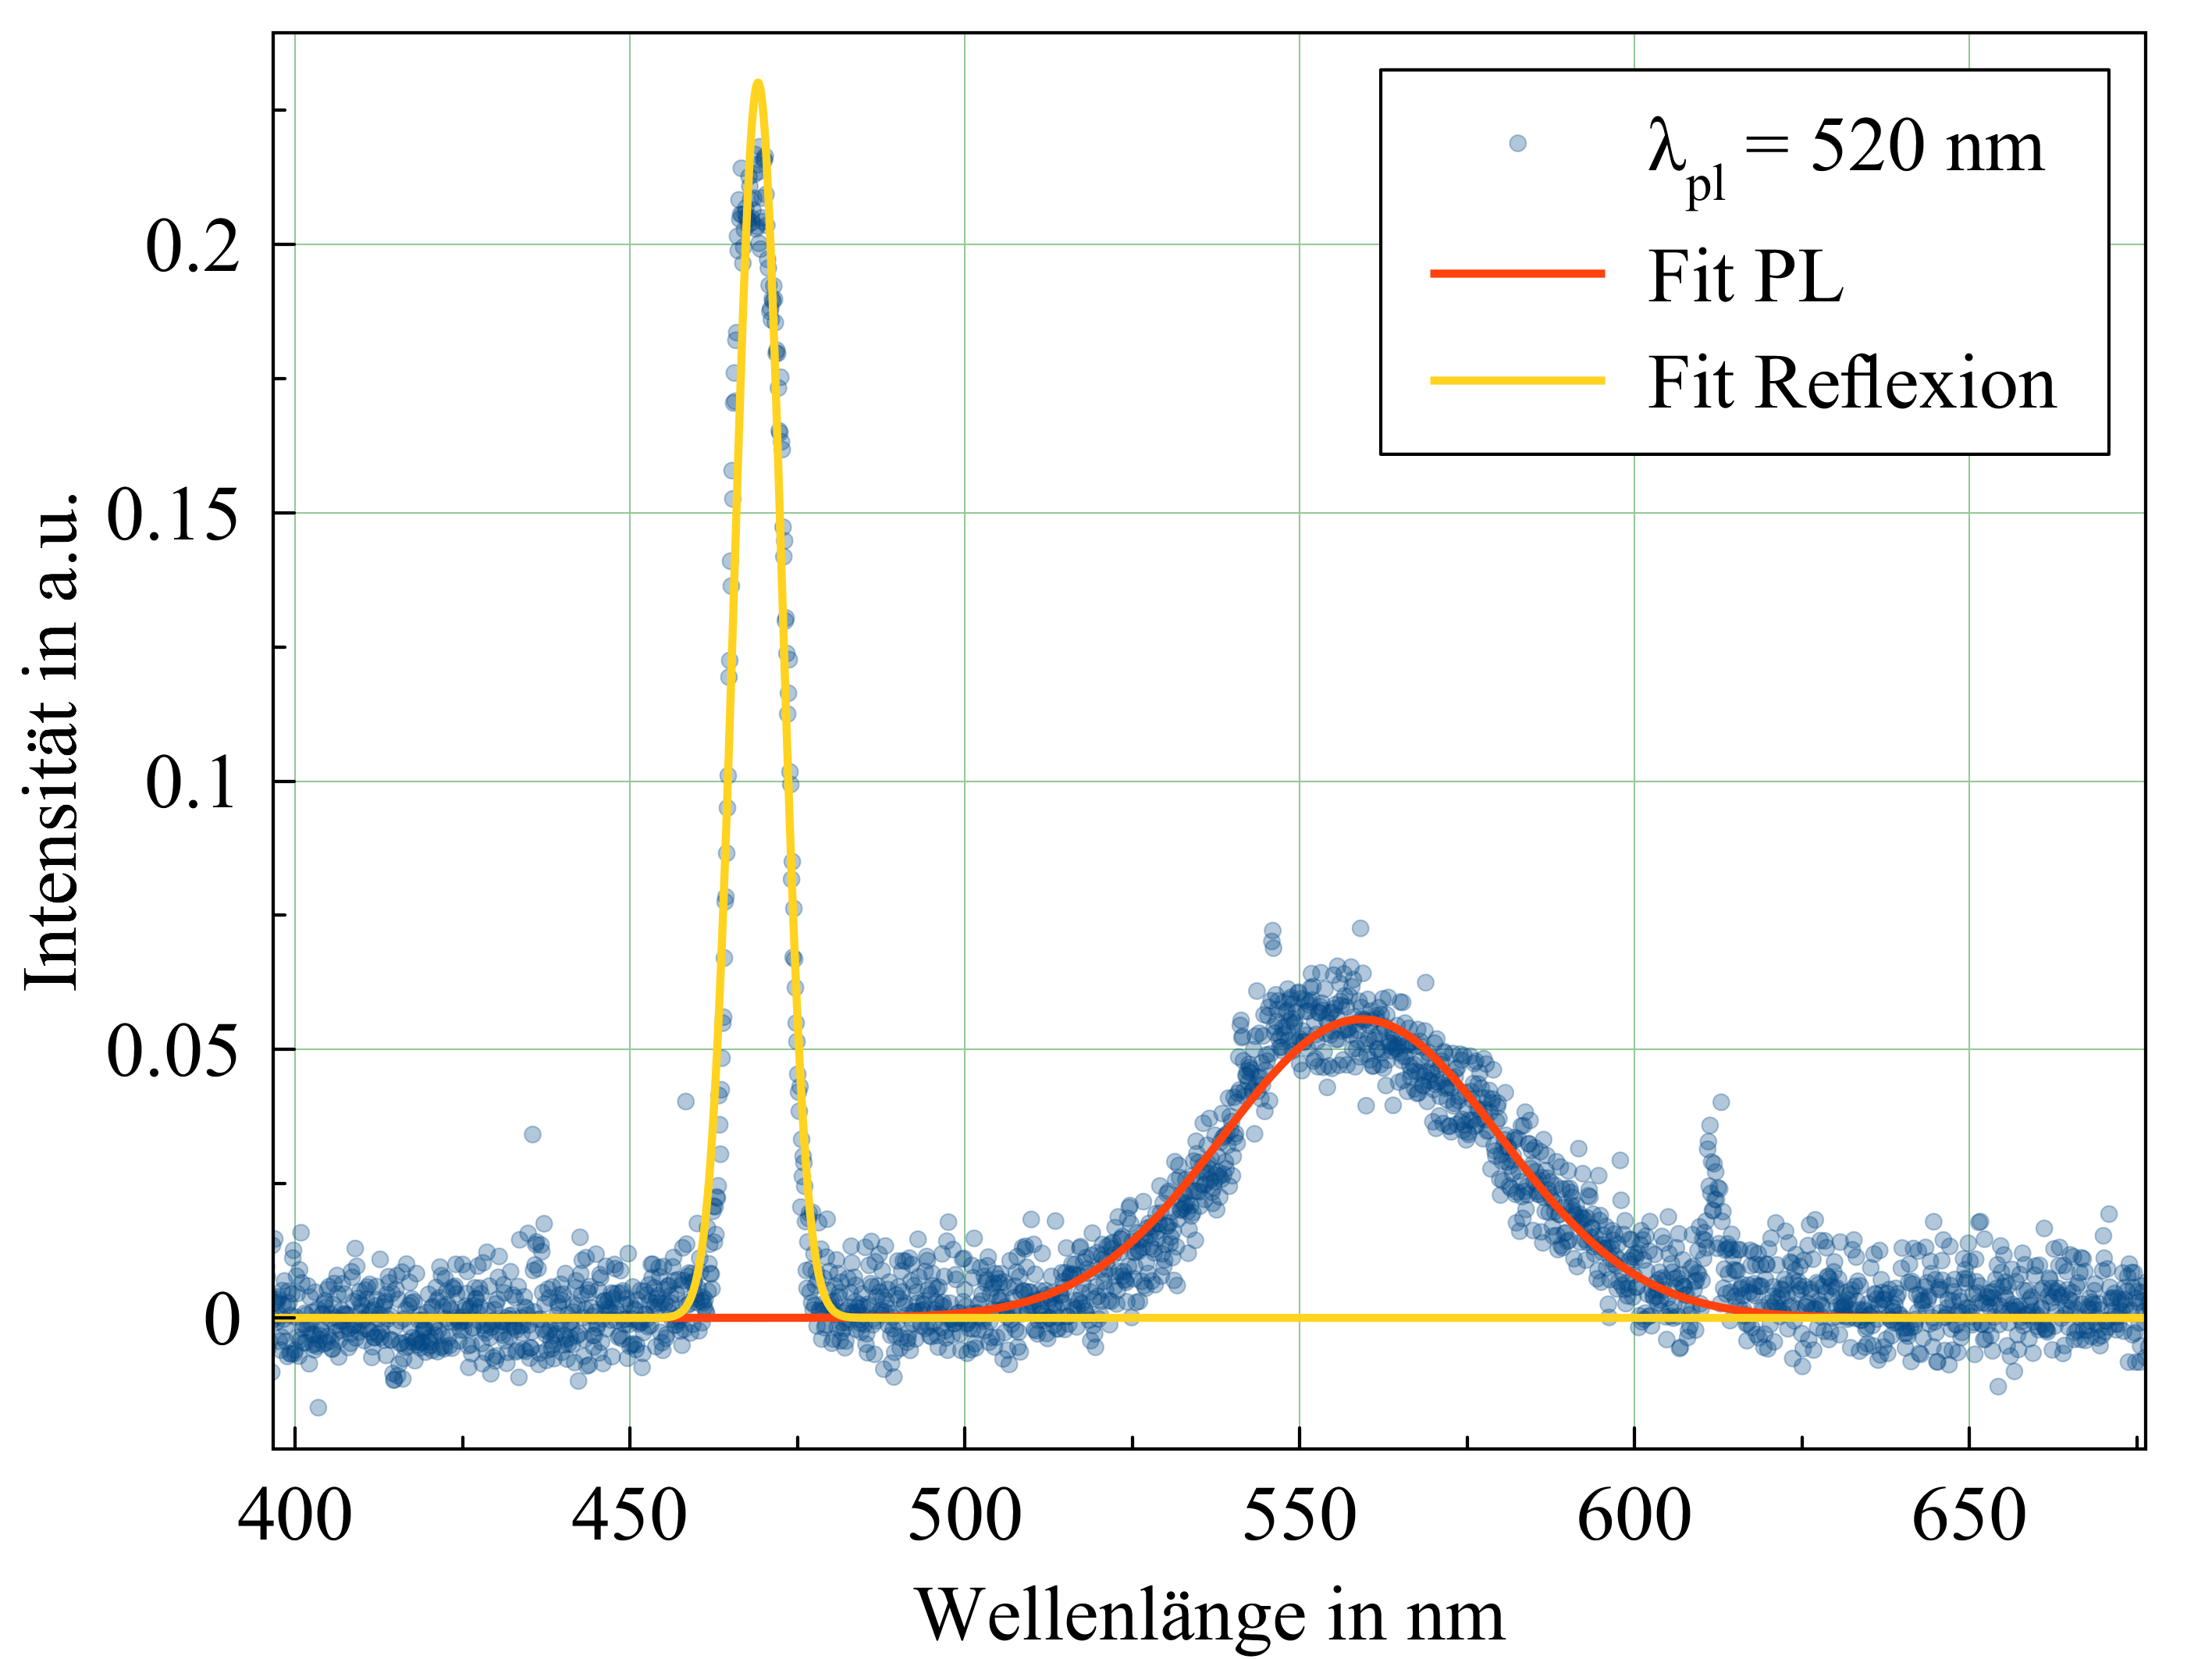
\includegraphics[width=\textwidth]{plots/Weisslicht_520_470.png}
    \caption{$\lambda=\SI{470}{\nano\meter}$}
  \end{subfigure}
  \caption{Photolumineszenzspektrum der $\lambda_{\text{PL}}=\SI{520}{\nano\meter}$ Probe.}
  \label{fig:PL_520}
\end{figure}
